\documentclass[]{DissertateUSU}
\usepackage{lmodern}
\usepackage{amssymb,amsmath}
\usepackage{ifxetex,ifluatex}
\usepackage{fixltx2e} % provides \textsubscript
\ifnum 0\ifxetex 1\fi\ifluatex 1\fi=0 % if pdftex
  \usepackage[T1]{fontenc}
  \usepackage[utf8]{inputenc}
\else % if luatex or xelatex
  \ifxetex
    \usepackage{mathspec}
  \else
    \usepackage{fontspec}
  \fi
  \defaultfontfeatures{Ligatures=TeX,Scale=MatchLowercase}
\fi
% use upquote if available, for straight quotes in verbatim environments
\IfFileExists{upquote.sty}{\usepackage{upquote}}{}
% use microtype if available
\IfFileExists{microtype.sty}{%
\usepackage{microtype}
\UseMicrotypeSet[protrusion]{basicmath} % disable protrusion for tt fonts
}{}
\usepackage[top=1in,bottom=1in,right=1in,left=1.5in]{geometry}
\usepackage{hyperref}
\hypersetup{unicode=true,
            pdftitle={Towards a Framework for Operational Risk in the Banking Sector},
            pdfauthor={Mphekeleli Hoohlo},
            pdfborder={0 0 0},
            breaklinks=true}
\urlstyle{same}  % don't use monospace font for urls
\usepackage{color}
\usepackage{fancyvrb}
\newcommand{\VerbBar}{|}
\newcommand{\VERB}{\Verb[commandchars=\\\{\}]}
\DefineVerbatimEnvironment{Highlighting}{Verbatim}{commandchars=\\\{\}}
% Add ',fontsize=\small' for more characters per line
\usepackage{framed}
\definecolor{shadecolor}{RGB}{248,248,248}
\newenvironment{Shaded}{\begin{snugshade}}{\end{snugshade}}
\newcommand{\KeywordTok}[1]{\textcolor[rgb]{0.13,0.29,0.53}{\textbf{#1}}}
\newcommand{\DataTypeTok}[1]{\textcolor[rgb]{0.13,0.29,0.53}{#1}}
\newcommand{\DecValTok}[1]{\textcolor[rgb]{0.00,0.00,0.81}{#1}}
\newcommand{\BaseNTok}[1]{\textcolor[rgb]{0.00,0.00,0.81}{#1}}
\newcommand{\FloatTok}[1]{\textcolor[rgb]{0.00,0.00,0.81}{#1}}
\newcommand{\ConstantTok}[1]{\textcolor[rgb]{0.00,0.00,0.00}{#1}}
\newcommand{\CharTok}[1]{\textcolor[rgb]{0.31,0.60,0.02}{#1}}
\newcommand{\SpecialCharTok}[1]{\textcolor[rgb]{0.00,0.00,0.00}{#1}}
\newcommand{\StringTok}[1]{\textcolor[rgb]{0.31,0.60,0.02}{#1}}
\newcommand{\VerbatimStringTok}[1]{\textcolor[rgb]{0.31,0.60,0.02}{#1}}
\newcommand{\SpecialStringTok}[1]{\textcolor[rgb]{0.31,0.60,0.02}{#1}}
\newcommand{\ImportTok}[1]{#1}
\newcommand{\CommentTok}[1]{\textcolor[rgb]{0.56,0.35,0.01}{\textit{#1}}}
\newcommand{\DocumentationTok}[1]{\textcolor[rgb]{0.56,0.35,0.01}{\textbf{\textit{#1}}}}
\newcommand{\AnnotationTok}[1]{\textcolor[rgb]{0.56,0.35,0.01}{\textbf{\textit{#1}}}}
\newcommand{\CommentVarTok}[1]{\textcolor[rgb]{0.56,0.35,0.01}{\textbf{\textit{#1}}}}
\newcommand{\OtherTok}[1]{\textcolor[rgb]{0.56,0.35,0.01}{#1}}
\newcommand{\FunctionTok}[1]{\textcolor[rgb]{0.00,0.00,0.00}{#1}}
\newcommand{\VariableTok}[1]{\textcolor[rgb]{0.00,0.00,0.00}{#1}}
\newcommand{\ControlFlowTok}[1]{\textcolor[rgb]{0.13,0.29,0.53}{\textbf{#1}}}
\newcommand{\OperatorTok}[1]{\textcolor[rgb]{0.81,0.36,0.00}{\textbf{#1}}}
\newcommand{\BuiltInTok}[1]{#1}
\newcommand{\ExtensionTok}[1]{#1}
\newcommand{\PreprocessorTok}[1]{\textcolor[rgb]{0.56,0.35,0.01}{\textit{#1}}}
\newcommand{\AttributeTok}[1]{\textcolor[rgb]{0.77,0.63,0.00}{#1}}
\newcommand{\RegionMarkerTok}[1]{#1}
\newcommand{\InformationTok}[1]{\textcolor[rgb]{0.56,0.35,0.01}{\textbf{\textit{#1}}}}
\newcommand{\WarningTok}[1]{\textcolor[rgb]{0.56,0.35,0.01}{\textbf{\textit{#1}}}}
\newcommand{\AlertTok}[1]{\textcolor[rgb]{0.94,0.16,0.16}{#1}}
\newcommand{\ErrorTok}[1]{\textcolor[rgb]{0.64,0.00,0.00}{\textbf{#1}}}
\newcommand{\NormalTok}[1]{#1}
\usepackage{graphicx,grffile}
\makeatletter
\def\maxwidth{\ifdim\Gin@nat@width>\linewidth\linewidth\else\Gin@nat@width\fi}
\def\maxheight{\ifdim\Gin@nat@height>\textheight\textheight\else\Gin@nat@height\fi}
\makeatother
% Scale images if necessary, so that they will not overflow the page
% margins by default, and it is still possible to overwrite the defaults
% using explicit options in \includegraphics[width, height, ...]{}
\setkeys{Gin}{width=\maxwidth,height=\maxheight,keepaspectratio}
\IfFileExists{parskip.sty}{%
\usepackage{parskip}
}{% else
\setlength{\parindent}{0pt}
\setlength{\parskip}{6pt plus 2pt minus 1pt}
}
\setlength{\emergencystretch}{3em}  % prevent overfull lines
\providecommand{\tightlist}{%
  \setlength{\itemsep}{0pt}\setlength{\parskip}{0pt}}
\setcounter{secnumdepth}{0}
% Redefines (sub)paragraphs to behave more like sections
\ifx\paragraph\undefined\else
\let\oldparagraph\paragraph
\renewcommand{\paragraph}[1]{\oldparagraph{#1}\mbox{}}
\fi
\ifx\subparagraph\undefined\else
\let\oldsubparagraph\subparagraph
\renewcommand{\subparagraph}[1]{\oldsubparagraph{#1}\mbox{}}
\fi

%%% Use protect on footnotes to avoid problems with footnotes in titles
\let\rmarkdownfootnote\footnote%
\def\footnote{\protect\rmarkdownfootnote}

%%% Change title format to be more compact
\usepackage{titling}

% Create subtitle command for use in maketitle
\newcommand{\subtitle}[1]{
  \posttitle{
    \begin{center}\large#1\end{center}
    }
}

\setlength{\droptitle}{-2em}

  \title{Towards a Framework for Operational Risk in the Banking Sector}
    \pretitle{\vspace{\droptitle}\centering\huge}
  \posttitle{\par}
    \author{Mphekeleli Hoohlo}
    \preauthor{\centering\large\emph}
  \postauthor{\par}
    \date{}
    \predate{}\postdate{}
  
\newcommand{\yeardegree}{ 2019 } \newcommand{\degree}{ Doctor of Philosophy }
 \newcommand{\field}{ Risk Theory (Finance) }
 \newcommand{\chairperson}{ Eric Schaling, Ph.D. }
 \newcommand{\committeeone}{ Thanti Mthanti, Ph.D. }
 \newcommand{\committeetwo}{ Odongo Kodongo, Ph.D. }
 \newcommand{\committeethree}{ Thabang Mokoaleli-Mokoteli, Ph.D. }
 \newcommand{\committeefour}{ Christopher Malikane, Ph.D. }
 \newcommand{\gradschoolguy}{ Paul Alagidede, Ph.D. }
 % Tables
      \usepackage{booktabs}
      \usepackage{threeparttable}
      \usepackage{array}
      \newcolumntype{x}[1]{%
      >{\centering\arraybackslash}m{#1}}%
      \usepackage{placeins}
      \usepackage{chngcntr}
      \counterwithin{figure}{chapter}
      \counterwithin{table}{chapter}
      \usepackage[makeroom]{cancel}

\begin{document}
\maketitle

\pagenumbering{roman} \pagestyle{empty} \copyrightpage

\newpage

\pagestyle{fancy} \fancyhead[L]{Abstract} \fancyhead[R]{\thepage}
\fancyfoot[C]{} \chapter*{ABSTRACT}
\addcontentsline{toc}{section}{Abstract}

\doublespacing

\begin{center}
Towards a Framework for Operational Risk \\ 
in the Banking Sector \\
\vspace{12pt}
by \\
\vspace{12pt}
Mphekeleli Hoohlo \\
University of the Witwatersrand, 2019
\end{center}

\vspace{12pt}

\singlespacing
\noindent Major Professor: Eric Schaling, Ph.D. \noindent Co-supervisor:
Thanti Mthanti, Ph.D.

\noindent Department: Law, Commerce \& Management

\vspace{12pt}

\doublespacing

The purpose of this research is to provide clarity; based on theory and
empirical evidence, on what the specific problems in the
\emph{operational risk} (OpRisk) literature are, given how its
importance has increased significantly over the last decades. There have
been a series of destructive events that have threatened the stability
of the financial system due to (OpRisk). In most, if not all of these
cases, human error is at the center of the chain of events that lead or
may lead to (OpRisk) losses. There are many attitudes that can
potentially infect organisational processes, the most persistent of
these attitudes stem from human failings that are exploitable Barberis
and Thaler (2003), thus forming a basis for the theoretical foundation
of \texttt{OpRisk}.

Shefrin (2016) notes that people would rather incur greater risks to
hold on to things they already have, than the risks they would taken to
get into that position in the first place, thereby risking a banks'
survival, rather than expose their trading losses by consciously
deceiving senior management to hide unethical operational practices. In
this paper the application of machine learning techniques on the
observed data demonstrates how these issues can be resolved given their
flexibility to different types of empirical data.

\hspace{11 cm} (128 pages)

\singlespacing

\newpage

\fancyhead[L]{Public Abstract} \fancyhead[R]{\thepage} \fancyfoot[C]{}
\chapter*{PUBLIC ABSTRACT}
\addcontentsline{toc}{section}{Public Abstract}

\doublespacing

\begin{center}
Towards a Framework for Operational Risk \\ 
in the Banking Sector \\
Mphekeleli Hoohlo
\end{center}

\vspace{12pt}

The purpose of this research is to provide clarity; based on theory and
empirical evidence, on what the specific problems in the
\emph{operational risk} (OpRisk) literature are, given how its
importance has increased significantly over the last decades. There have
been a series of destructive events that have threatened the stability
of the financial system due to (OpRisk). In most, if not all of these
cases, human error is at the center of the chain of events that lead or
may lead to (OpRisk) losses. There are many attitudes that can
potentially infect organisational processes, the most persistent of
these attitudes stem from human failings that are exploitable Barberis
and Thaler (2003), thus forming a basis for the theoretical foundation
of \texttt{OpRisk}.

Shefrin (2016) notes that people would rather incur greater risks to
hold on to things they already have, than the risks they would taken to
get into that position in the first place, thereby risking a banks'
survival, rather than expose their trading losses by consciously
deceiving senior management to hide unethical operational practices. In
this paper the application of machine learning techniques on the
observed data demonstrates how these issues can be resolved given their
flexibility to different types of empirical

\singlespacing

\newpage

\fancyhead[L]{Dedication} \fancyhead[R]{\thepage} \fancyfoot[C]{}
\chapter*{DEDICATION} \addcontentsline{toc}{section}{Dedication}

This work---the dissertation and all work associated with it---is
dedicated to \ldots. I will always be grateful to her and for her. I
also dedicate this work to my child, who patiently loved a father who
was often busy working, even when at home. Finally, I dedicate this work
to my parents and siblings, who kept me level-headed throughout the
process, providing wise and thoughtful advice.

This work is truly evidence of the love I am surrounded by.

\hspace{10.5 cm} \emph{Mphekeleli Hoohlo}

\newpage

\fancyhead[L]{Acknowledgments} \fancyhead[R]{\thepage} \fancyfoot[C]{}
\chapter*{ACKNOWLEDGEMENTS}
\addcontentsline{toc}{section}{Acknowledgments}

Several individuals deserve recognition for their help in this work.
First, I am greatly indebted to Dr.~Ginger Lockhart for giving me the
opportunity to find where my research passions are---especially
quantitatively. She provided guidance in my budding career with the
right amount of understanding and pressure to push me to be a more
productive and capable researcher. I also owe a great deal to
Dr.~Jamison Fargo, for many, many reasons including helping me get into
the program when my application was delayed. He has also proven to be an
important mentor and friend. Relatedly, I am grateful to Dr.~Karl White
in allowing me to become his first student in many years, providing
opportunities to develop as a researcher in an important field.

My friends and colleagues in the program also deserve serious
recognition for their help and support. Specifically, Dr.~Emily Brignone
played an invaluable role as a leader and friend as I pursued my goals
in the program. She provided timely and important help throughout the
process. I appreciate her loyal, honest, genuine friendship. Another
good friend that deserved mentioning is Sara Doutré, who also provided
support and laughs when I needed it (and sometimes when I did not need
it but still welcomed it!). My friends in the Prevention Science Lab
continually offered support and collaboration that made my job easier
and more enjoyable.

I also want to acknowledge my committee, in providing feedback,
guidance, and support throughout my graduate student career. The
department's and college's administrative staff and heads, although
working in the background, were a huge help in getting me to where I am
today. Finally, Utah State University as a school has proven to be a
fantastic place to grow academically and to mature into a researcher.

\newpage

\fancyhead[L]{Table of Contents} \fancyhead[R]{\thepage} \fancyfoot[C]{}
\tableofcontents

\newpage

\fancyhead[L]{List of Tables} \fancyhead[R]{\thepage} \fancyfoot[C]{}
\listoftables

\newpage

\fancyhead[L]{List of Figures} \fancyhead[R]{\thepage} \fancyfoot[C]{}
\listoffigures

\newpage

\pagenumbering{arabic}

\newpage

\fancyhead[L]{Introduction} \fancyhead[R]{\thepage} \fancyfoot[C]{}

\chapter{INTRODUCTION}

\doublespacing

\textbf{\section{Purpose of the study}} \label{sec:Purpose of the study}

The purpose of this research is to apply a generalised linear model
(GLM) suitable for exposure-based operational risk (EBOR) treatments
within the operational risk management framework (ORMF), effectively
replacing historical loss severity curves obtained from historical loss
counts, by forward-looking measures using event frequencies based on
actual operational risk (OpRisk) exposures. Preliminary work on EBOR
models was undertaken by (Einemann, Fritscher, and Kalkbrener, 2018).
Secondly, this study provides a comprehensive computational comparison
of various data-intensive techniques amongst each other, and versus
\emph{classical} statistical estimation methods for classification and
regression performances.\medskip

Our understanding of existing ORMF to date is limited to the assumption
that financial institutions (FI's) are risk-neutral. Thirdly, in lieu of
the afore-mentioned, this study finally seeks to invalidate the
risk-neutral assumption, by means of various unsupervised learning
techniques, by proposing that FI's are more risk-averse; this can be
measured by analysing subtle patterns between data features and trends
in the allocated risk capital estimates. In theory, a risk manager who
experiences persistent/excessive losses due to particular risk events,
would over-compensate cover for these particular risk types, and this
would show in reduced losses in these types over time.

\textbf{\section{The theoretical foundation of OpRisk}}
\label{sec:The theoretical foundation of OpRisk}

Most banks' estimates for their risk are divided into credit risk
(50\%), market risk (15\%) and OpRisk (35\%). Cruz (2002) postulated
that OpRisk, which focuses on the human side of risk management is
difficult to manage with the reduced ability to measure it. The process
of OpRisk, that is, the how manifests in conscious and/or unconscious
states of the risk manager/s (Hemrit and Arab, 2012), and encompasses
approaches and theories that focus on how one will choose when faced
with a decision, based on how comfortable they are with the situation
and the variables that are present.

\subsection{Definition of operational risk}
\label{ssec:Definition of operational risk}

Operational risk (OpRisk) is defined as:
\emph{The risk of loss resulting from inadequate or failed internal processes, people and systems, and from external events. This definition includes legal risk, but excludes strategic and reputational risk.}(Risk,
2001).\medskip

A major managerial concern for businesses is an inability to identify
and account for their susceptibility to OpRisk events following a number
of very costly and highly publicized operational losses, in particular,
it became popular following a fraudulent trading incident which was
responsible for a catastrophic loss that lead to the collapse of Barings
Bank (the UK's oldest bank) in 1995.\medskip

The term OpRisk began to be used after the afore-mentioned and similar
types of OpRisk events became more common. A (rogue) trader (Nick
Leeson), who risked the banks' survival rather than expose his trading
losses, by consciously deceiving senior management to hide his unethical
acts, was found to have been responsible for unethical trading practices
when he created illegal trades in his account, then used his position in
the front and back offices of the bank to hide his trading losses. Worse
still, he incurred a greater risk to the bank by lying in order to give
a false impression of his profits. Shefrin (2016) notes that people
would rather incur greater risks to hold on to things they already have,
than the risks they would taken to get into that position in the first
place.\medskip

It was later discovered that he was placing illegal bets in the
Asian-markets, and kept these contracts out of sight from senior
management to cover up his illegal activity. When his fraudulent
behaviour was discovered (after an earthquake hit at Kobe in Japan, that
collapsed the Osaka Securities Exchange) he succumbed to unrecoverable
losses due to trading positions he had accumulated, which resulted in a
loss of around \pounds 1.3 billion to the bank, thus resulting in it's
collapse. In most, if not all of these cases, human error is at the
center of the chain of events that lead or may lead to OpRisk
losses.\medskip\medskip

Since then, there have been a series of destructive events that have
threatened the stability of the financial system due to OpRisk. Large
fines have been imposed on the culprits and regulatory scrutiny has been
heightened as a result of a number of operational events, e.g.~the
January 2016 \lq\lq Dark Pool\rq\rq~trading penalties suffered by
Barclays (\$70mn) and Credit Suisse (\$85mn), imposed by the United
States (US) based securities exchange commision (SEC). These OpRisk loss
events were due to fraudulent trading activity consisting of rogue
traders dealing in illegally placed high frequency trades for private
clients where prices were hidden.\medskip 

In South Africa (SA), there is an upcoming case of price fixing and
market allocation in trading foreign exchange (FX) currency pairs,
reffered to the SA based competition tribunal for prosecution. Absa
bank, Standard bank \& Investec may be liable to payment of an
admistrative penalty equal to 10\% of their annual turnover in 2016,
following accusations by the local based competition commission in
February 2017, of rogue traders manipulating the price of the rand
through buying and selling US dollars in exchange for the rand at fixed
prices. According to the competition commission, it has been alleged
that currency traders have been colluding or manipulating the price of
the rand through these buy and sell orders to change supply of the
currency.\medskip

This has compromised the quality and accuracy of risk management's
advisory service and pedigree, and aroused huge interest as the value of
the rand has implications on South African's. Furthermore, this kind of
behaviour can lead to catastrophic operational losses, as with the case
for the Barings event, resulting is a mismatch between business'
expectations and the value the risk management practice was able to
deliver, which is prevalent across FI's and remains unchanged. There are
many attitudes that can potentially infect organisational processes, the
most persistent of these attitudes stem from human failings that are
exploitable (Barberis and Thaler, 2003); i.e.~humans' propensity to be
deceitful during periods of distress, thus forming a basis for a
theoretical foundation of OpRisk management.

\textbf{\section{Basel Committee's quantitative operational risk management framework}}
\label{sec:Basel Committee's quantitative operational risk management framework}

The Bank for International Settlements (BIS) is an organisation
consisting of a group of central bank governors and heads of supervision
of central banks around the world who represent an authority on good
risk management in banking. More specifically, the BIS oversee the
duties of the Basel Committee on Banking Supervision (BCBS)/Basel
Commitee. The role of the BCBS is to set out guidelines on international
financial regulation to cover risks in the banking sector. There have
been three banking accords from the BCBS under the supervision of the
BIS in dealing with financial regulation, viz., Basel I, Basel II \&
Basel III. These accords describe an overview of capital requirements
for financial institutions (FI's) in order to create a level playing
field, by making regulations uniform throughout the world.\medskip 

\subsection{The Capital Adequacy Accord (Basel I)}

Basel I was established in 1988. Basel I meant that FI's were required
to assign capital for credit risk to protect against credit default. In
1996, an amendment to Basel I imposed additional requirements to cover
exposure due to market risk as well as credit risks. Basel I effectively
minimised rules that favoured local FI's over potential foreign
competitors, by opening up global competition so that these banks could
buffer against international solvency. In 2001, the Risk (2001)
consultative package provided an overview of the proposed framework for
regulatory capital (RC) charge for OpRisk. A fiancial institution (FI)
has an OpRisk component, which constitutes a substantial risk component
other than credit and market risk. There are two types of OpRisk's viz.,
potential high severity risk where the probability of an extreme loss is
very small but costly, and high frequency/low severity risk where
frequency plays a major role in the OpRisk capital charge
calculation.\medskip 

\subsection{New Capital Adequacy Accord (Basel II)}

The framework for Basel II was implemented in June 2006. Basel II
introduces more restrictive capital charge measures with specific
emphasis on OpRisk. Under Basel II OpRisk loss events (i.e.~a default in
the credit risk jargon) are categorised under seven event types. e.g.,
Process Risk is one such category and is usually responsible for most
OpRisk events, it is the risk that operational losses/problems would
take place in the banks transactions.\medskip

Regarding the sequence Basel I and Basel II: Regulation begins as a
qualitative recommendation which requires banks to have an
assets-to-capital multiple of at least 20, then focuses on ratios in
which both on-balance sheet and off-balance sheet items are used to
calculate the bank's total risk-weighted assets
(RWA's)\footnote{Also reffered to as risk-weighted amount, it is a measure of the bank's total credit exposure},
then on tail risk. In other words, auditors' discretion is replaced by
market perception of capital, meaning there is a market risk capital
charge for all items in the trading business line, then exciting new
static risk management approaches which involve calculating a 99.9
percentile left tail confidence interval to measure OpRisk value-at-risk
(VaR) and convert it into a RC charge.\medskip 

\subsection{Basel III}

Basel III establishes tougher capital standards through more restrictive
capital definitions, higher RWA's, additional capital buffers, and
higher requirements for minimum capital ratios (Dorval, 2013). Through
Basel III, the BCBS is introducing a number of fundamental reforms
grouped under three main headings (Committee and others, 2010): 1{]} A
future of more capital through incremental trading book risk (credit
items in trading book treated in the same way as if they were in banking
book), 2{]} More liquidity through the introduction of a global
liquidity risk standard (Basel III will push banks toward holding
greater levels of liquid instruments, such as government bonds and more
liquid corporate instruments), and 3{]} Lower risk under the new
requirements of the capital base, i.e., establish more standardized
risk-adjusted capital requirements.\medskip

The future regulatory environment requires OpRisk professionals, who are
not only intelligent, creative and motivated but also have the courage
to uphold the OpRisk advisory service standards. Businesses that want to
successfuly manage risk, would be well advised to utilize new
theoretical and empirical techniques, such that large and small scale
experiments play an important role in risk analysis and regulatory
research.

\textbf{\section{modern OpRisk measurement frameworks (ORMF's)}}
\label{sec:modern OpRisk measurement frameworks (ORMF's)}

Basel II describes three methods of calculating capital charge for
OpRisk RC viz., the standardised approach (SA), the basic indicator
approach (BIA) and the internal measurement approach (IMA). The basic
indicator approach (BIA) sets the OpRisk RC equal to a percentage (15\%)
of the annual gross income of the firm as a whole to determine the
annual capital charge. The SA is similar to the BIA except the firm is
split into eight business lines and assigned a different percentage of a
three year average gross income per business line, the summation of
which is the capital charge (Hoohlo, 2015). In the IMA, the bank uses
it's own internal models to calculate OpRisk loss.\medskip

\subsection{Advanced Measurement Approach (AMA)}

The advanced measurement approach (AMA) is an IMA method which applies
estimation techniques of OpRisk capital charge derived from a bank's
internal risk measurement system Cruz (2002). Basel II proposed
measurement of OpRisk to define capital requirements against unexpected
bank losses whereas the unexpected loss (UL) is the quantile for the
level \(\alpha\) minus the mean. According to the AMA, which is thought
to outperform the simpler SA approach and the BIA, RC requirements are
defined according to the UL limit in one year and the loss distribution
at a 99.9\% confidence level (\(\alpha = 0.01\%\)) aggegate loss
distribution\footnote{The aggregate loss distribution is obtained by convoluting a loss event frequency distribution and a loss severity distribution by means of the random sums method.}
used as a measure of RC. The BCBS proposes to define RC as \(RC = UL\).
This involves simulations based on historical data to establish
frequency and severity distributions for losses. In this case the RC is
a VaR measure.\medskip

The Basel III capital adequacy rules permit model-based calculation
methods for capital, including the AMA for OpRisk capital. Under Basel
III, standardised methods for OpRisk capital have been overhauled,
however for a while there was no prospect of an overhaul of the AMA.
Given the relative infancy of the field of OpRisk measurement, banks are
mostly free to choose among various AMA principle-based frameworks to a
significant degree of flexibility (Risk, 2016). A bank that undertakes
an AMA should be able to influence their capital requirements through
modeling techniques resulting in lowered pressure on OpRisk capital
levels, which in turn has a positive impact on the bank.\medskip

A FI's ability to determine the framework used for its regulatory OpRisk
RC calculation, evolves from how advanced the FI is along the spectrum
of available approaches used to determine capital charge (Risk, 2001).
BCBS recognizes that a variety of potentially credible approaches to
quantify OpRisk are currently being developed by the industry, and that
these R\&D activities should be incentivised. Increasing levels of
sophistication of OpRisk measurement methodologies should generally be
rewarded with a reduction in the regulatory OpRisk capital requirement.

\subsection{The standardised measurement approach (SMA)}

The flexibility of internal models was expected to narrow over time as
more accurate OpRisk measurement was obtained and stable measures of RC
were reached, ultimately leading to the emergence of best practice.
Instead, internal models produced wildly differing results of OpRisk RC
capital from bank to bank, contrary to the expectations of the BCBS. In
March 2016, the BCBS published for consultation a standardised
measurement approach (SMA) for OpRisk RC; that proposes to abandon the
freedom of internal modelling (thus ending the AMA) approaches for
OpRisk RC, in exchange for being able to use a simple formula to
facilitate comparability across the industry.\medskip

Under the SMA, RC will be determined using a simple method comprising of
two components: A stylised systemic risk model (business indicator
component), and an idiosyncratic risk model (loss component), which are
combined via an internal loss multiplier (ILM), whose function is to
link capital to a FI's operational loss experience to determine SMA
capital.\medskip

The SMA formula is thought to be consistent with regulators' intent for
simplification and increased comparability across most banks. However,
there is a feeling from some in the banking industry that the SMA is
disadvantaged as it is not the same as measuring OpRisk. Mignola,
Ugoccioni, and Cope (2016) and Peters, Shevchenko, Hassani, and Chapelle
(2016) identified that the SMA does not respond appropriately to changes
in the risk profile of a bank i.e., it is unstable viz., two banks of
the same risk profile and size can exibit OpRisk RC differences
exceeding 100\%, and risk insensitive; that SMA capital results
generally appear to be more variable across banks than AMA results,
where banks had the option of fitting the loss data to statistical
distributions.

\subsection{Argument}
\label{ssec:Argument}

Over the last twenty years, hard-won incremental steps to develop a
measure for the size of OpRisk exposure along with the emergence of
promising technologies presents a unique opportunity for bankers and
treasurers - traditionally risk-averse players - to develop a novel type
of way of looking at decision making under risk/uncertainty. New
technologies have been introduced which make use of up to date technical
solutions (such as homo heuristics developed by Gigerenzer and Brighton
(2009), who mainatain their methods solve practical finance problems by
simple rules of thumb, or Kahneman (2003)'s intuitive judgements and
deliberate decision making), argued to more likely represent the true
embedded OpRisk in financial organisations as these methods are designed
to fit normal behavioral patterns in their formulation, which is
consistent with how decisions are made under risk/uncertainty.\medskip 

What are the important steps toward completing the post crisis reforms
during the current year? Should the risk management fraternity follow
the
chartered\footnote{Meaning as of the publication [@risk2016supporting] the methods brought forth in the consultative document have not been approved for the public, the ideas within an experimental (leased) phase for the exclusive use of BCBS and certain FI's}
path followed in the Risk (2016) consultative document, scrapping away
twenty years of internal measurement approaches (such as the AMA), or
should the focus of financial regulators shift toward improving on what
they see fit within current existing AMA frameworks. The question is
should OpRisk managements' focus be on stimulating active discussions on
practical approaches to quantify, model and manage OpRisk for better
risk management and improved controls, or abandon the adoption of
innovative measurement approaches, such as the AMA, in exchange for
being able to use a simple formula across the whole industry?\medskip 

\textbf{\section{Context of the study}} \label{sec:Context of the study}

Regulatory reforms are designed and fines imposed to protect against
operational errors and other conduct costs connected with wrongdoing and
employee misconduct. Despite the introduction and use of these seemingly
robust strategies, regulations, processes and practices relating to
managing risk in FI's, bank losses continue to occur at a rather
distressing frequency. A cyclical pattern of OpRisk loss events still
persists; as evidenced in the recent price fixing and collusion cases,
defeating the explicit objectives of risk management frameworks. This
demonstrates a scourge of reflexivity prevailing in financial markets
emphasising that, there are theories that seem to work for a time only
to outlive their use and become insufficient for the complexities that
arise in reality.\medskip 

\subsection{Why \texttt{OpRisk?}}

A forceful narrative in management theory is that an organisation
running effective maintenance procedures combined with optimal team and
individual performers i.e., the right balance of skills in the labour
force and adequate technological advancements, means systems and
services can be used to more efficiently produce material gains, enhance
organisational effectiveness, meet business objectives and increase
investment activity. Conversely, the risk of the loss of business
certainty associated with lowered organisational competitiveness and
inadequate systems technology that underpins operations and services is
a key source leading to a potential breakdown in investment services
activity (Hoohlo, 2015). In fact OpRisk control could set banks apart in
competition. This serves as an incentive to support regulation,
particularly Basel III recovery and resolution processes.\medskip

Consider the case of a regulator in a financial system, who assumes that
he/she is consiously and accurately analysing an observed subject,
trusting the validity and relying on the visual information that their
sense of sight reveals. In the absence of visual confirmation they are
hindered from extracting and/or analysing information about the system
and their efforts to regulate could potentialy fail. The organisational
methods and functioning of current information systems in this industry
sector obscure the full extent of OpRisk challenges from the eyes of the
risk practitioner.\medskip 

When an attack such as an operational error occurs at a speed that the
OpRisk agent (an individual legal entity or a group) is unable to react
quickly enough, due to limitations of their processing speed, and they
are not able to process all the information in the given time span, they
could lose control/fail to comply with regulatory standards. The latter
case is more often than not the most accurate reflection of current risk
management practices. The agent represents one end of the spectrum of a
risk management strategy, which mitigates risk and enforces regulation,
dependent on the information recieved. The other end of the spectrum is
one which does not react at all to changes in the system
environment.\medskip 

Current conventional financial systems where information processing is
slow and have a tendency to rely on manual, uncertain, unpredictable and
unrealistic controls, obscure risk management reporting and produce
undesirable market conditions. The OpRisk management function should be
able to assist the firms' ability to mitigate risks by acquiring and/or
refining risk management solutions which deliver reliable and consistent
benefits of improved control and management of the risks inherent in
banking operations (Dorval, 2013). This proposal attempts to fill the
gap in the current system where there is a risk management information
lag or an obstruction from the eyes of the risk practitioner.

\textbf{\section{Analysis and interpretation issues with behavioral finance theory}}
\label{sec:Analysis and interpretation issues with behavioral finance theory}

Behavioral management theory is very much concerned with social factors
such as motivation, support and employee relations. A critical component
of behavioral finance is building models which better reflect actual
behavior. Studies have revealed that these social factors are not easy
to incorporate into finance models or to understand in the traditional
framework.\medskip 

The traditional finance paradigm seeks to understand financial markets
using models in which agents are \lq\lq rational\rq\rq. According to
Barberis and Thaler (2003), this means that agents update their beliefs
on the onset of new information, and that given their beliefs, they make
choices that are normatively acceptable, and that most people do this
most of the time. Neoclassical theory has grown to become the primary
take on modern-day economics formed to solve problems for decision
making under uncertainty/risk. Expected Utility Theory (EUT) has
dominated the analysis and has been generally accepted as the normative
model of rational choice, and widely applied as a descriptive model of
economic choice (Kahneman and Tversky, 2013).

\subsection{Expected utility theory}
\label{ssec:Expected utility theory}

Expected utility
theory\footnote{Expected utility theory provides a model of rationality based on choice.}
(EUT): We see a fundamental relation for expected utility (Expectation)
of a contract \(X\), that yields outcome \(x_i\) with probability
\(p_i\), where \(X = (x_1,p_1; ...; x_n,p_n)\) and
\(p_1+p_2+\ldots+p_n=1\) given by:

\singlespacing

\begin{equation}\label{EUT_extended}
U(x_1,p_1;\ldots;x_n,p_n) = p_1u(x_1)+\ldots+p_nu(x_n) 
\end{equation}

\doublespacing
corroborated by Morgenstern and Von Neumann (1953); Friedman and Savage
(1948); Kahneman and Tversky (2013) \& others.

A common thread running through the rational viz., the neoclassical take
of modern-day economics vs the non-neoclassical schools of thought are
findings of behavioral economics which tend to refute the notion that
individuals behave rationally. Many argue that individuals are
fundamentally irrational because they do not behave rationally giving
rise to a literature and debates as to which heuristics and sociological
and institutional priors are rational (Altman, 2008).\medskip

In the real world there is a point of transition between the traditional
(neoclassical) approach to decision making, based on data and data
anaysis (logic and rational), by adding new parameters and arguments
that are outside rational conventional thinking but are also valid. For
example, that neoclassical theory makes use of the assumption that all
parties will behave rationally overlooks the fact that human nature is
vulnerable to other forces, which causes people to make irrational
choices.\medskip 

An essential ingredient of any model trying to understand trading
behavior is an assumption about investor preferences (Barberis and
Thaler, 2003), or how investors evaluate risky gambles. Investors
systematically deviate from rationality when making financial decisions,
yet as acknowledged by Kuhnen and Knutson (2005), the mechanisms
responsible for these deviations have not been fully identified. Some
errors in judgement suggest distinct mental operations promote different
types of financial choices that may lead to investing mistakes.
Deviations from the optimal investment strategy of a rational risk
neutral agent are viewed as risk-seeking mistakes and risk-aversion
mistakes (Kuhnen and Knutson, 2005).\medskip 

\subsection{Theoretical investigations for the quantification of moderm ORMF}

Kuhnen and Knutson (2005) explain that these risk-seeking choices (such
as gambling at a casino) and risk-averse choices (such as buying
insurance) may be driven by distinct
neural\footnote{As recent evidence from human brain imaging has shown [@kuhnen2005neural] linking neural states to risk-related behaviours [@paulus2003increased].}
phenomena, which when activated can lead to a shift in risk preferences.
Kuhnen and Knutson (2005) found that certain areas of the brain precede
risk-seeking mistakes or risky choices and other areas precede
risk-aversion mistakes or riskless choices. A risk-aversion mistake is
one where a gamble on a prospect of a gain is taken by a risk-averse
agent in the face of the chance of a prospective loss. The fear of
losing prohibits one's urge to gamble, but people engage in gambling
activity anyway. Barberis and Thaler (2003) show that people regularly
deviate from the traditional finance paradigm evidenced by the extensive
experimental results compiled by cognitive psycologists on how people
make decisions given their beliefs.\medskip 

Kahneman and Tversky (2013) maintains, preferences between prospects
which violate rational behaviour demonstrate that outcomes which are
obtained with certainty are overweighted relative to uncertain outcomes.
This will contribute to a risk-averse preference for a sure gain over a
larger gain that is merely probable or a risk-seeking preference for a
loss that is merely probable over a smaller loss that it certain. As a
psycological principle, overweighting of certainty favours risk-aversion
in the domain of gains and risk-seeking in the domain of losses.\medskip

The present discussion replicates the common behavioral pattern of risk
aversion, where people weigh losses more than equivalent gains.
Furthermore, neuroeconomic research shows that this pattern of behavior
is directly tied to the brain's greater sensitivity to potential losses
than gains (Tom, Fox, Trepel, and Poldrack, 2007). This provides a
target for investigating a more comprehensive theory of individual
decision-making rather than the rational actor model and thus yield new
insights relevant to economic
theory\footnote{Representing ability of FI's financial market models to characterise the repeated decision-making process that applies to loss aversion}
(Kuhnen and Knutson, 2005).\medskip  

If people are reasonably accurate in predicting their choices, the
presence of systematic violations of risk neutral behavior provides
presumptive evidence against this i.e., people systematically violate
EUT when choosing among risky gambles. This seeks to improve and adapt
to reality and advance different interpretations of economic behaviour;
viz., to propose a more adequately descriptive model, that can represent
the basis for an alternative to the way the traditional model is built
for decisions taken under uncertainty. This has led some influential
commentators to call for an entirely new economic paradigm to displace
conventional neoclassical theory with a psycologically more realistic
preference specification (List, 2004).

\textbf{\section{A new class of ORMF models approach}}
\label{sec:A new class of ORMF models approach}

A substantial body of evidence shows that decision makers systematically
violate EUT when choosing between risky prospects. Indeed, people would
rather satisfy their needs than maximise their utility, contravening the
normative model of rational choice (i.e., EUT) which has dominated the
analysis of decision making under risk. In recent work (Barberis and
Thaler, 2003) in behavioral finance, it has been argued that some of the
lessons learnt from violations of EUT are central to understanding a
number of financial phenomena. In response to this, there has been
several theories put forward advocating for the basis of a slightly
different intepretation which describes how individuals actually make
decisions under uncertainty/risk. Of all the non-EUT's, we focus on
Prospect Theory (PT) as this framework has had most success matching
most empirical
facts\footnote{OpRisk loss events in FI's are largely due to human failings that are exploitable e.g., fraudulent trading activity, and PT is based on the same behavioural element of how people make financial decisions about prospects}.\medskip 

Kahneman and Tversky (2013) list the key elements of PT, which are 1{]}
a value function, and 2{]} a non-linear transformation of the
probability scale, that factors in risk aversion of the participants.
According to Kahneman and Tversky (2013), the probability scale
overweights small probabilities and underweights high probabilities.
This feature is known as loss/risk aversion: This means that people have
a greater sensitivity to losses (around 2.5 times more times) than
gains, and are especially sensitive to small losses unless accompanied
by small
gains\footnote{Diminishing marginal utility for gains but opposite for losses.}.
Loss aversion is a strong differentiator when it comes to explaining
exceptions to the general risk patterns that characterize prospect
theory.\medskip 

\subsection{Prospect theory}
\label{ssec:Prospect theory}

By relaxation of the expectation principle in equation
\ref{sssec:Expected utility theory}, the over-all value
\(\mathbf{\bigvee}\) of the regular prospect \((x,p;y,q)\): In such a
prospect, one receives \(x\) with probability \(p\), \(y\) with
probability \(q\), and nothing with probability \(1-p-q\), is expressed
in terms of two scales, \(\pi(\cdot)\), and \(\nu(\cdot)\), where
\(\pi(\cdot)\) is a decision weight and \(\nu(\cdot)\) a number
reflecting the subjective value of the outcome. Then
\(\mathbf{\bigvee}\) is assigned the value:

\begin{equation}\label{eqn2}
\mathbf{\bigvee}=\pi(p)\nu(x)+\pi(q)\nu(y) \qquad\mbox{iff} \qquad p+q \leq 1
\end{equation}

The scale, \(\pi\), associates with each probability \(p\) a decision
weight which reflects the impact of \(p\) on the over-all value of the
prospect. The second scale, \(\nu\), assigns to each outcome \(x\) a
number \(\nu(x)\), which measures the value of deviations from a
reference point i.e., gains or losses. \(\pi\) is not a probability
measure and \(\pi(p) + \pi(1-p) < 1\). Through PT we add new parameters
and arguments to improve the mathematical modelling method for decisions
taken under risk/uncertainty, such that the value of each outcome is
multiplied by a decision weight, not by an additive probability.

PT looks for common attitudes in people (in FI's) with regard to their
behaviour toward taking financial risks or gambles that cannot be
captured by EUT. In light of this view, people are not fully invested in
either of the percieved outcomes \(x\) and \(y\), Which tells us that
\(p+q \leq 1\). In lieu of this, an FI using (internal) historical
OpRisk loss data to model future events; say a historical case of fraud
at the FI occurs and is incorporated in the model, the probability of
making the same error in future is provided for in the model versus risk
events that haven't happened. The modelled future should over-provide
for the loss events that have already occured, which fits normal
patterns around individuals psycological make up and is consistent with
risk-averse behavior. The idea at the basis of PT is that a better
modeling method can be obtained which leads to a closer approximation of
the over-all-value of OpRisk losses.

\subsection{Modeling}

In this study, an important new algorithm for ORMFs and is laid out
coupled with data intensive estimation techniques; viz. Generalised
Additive Models for locatin Scale \& Shape (GAMLSS), Generalized Linear
Models (GLDs), Artificial Neural Networks (ANNs), Random Forest (RF) \&
Decision Trees (DTs), which have capabilities to tease out the deep
hierarchies in the features of covariates irrespective of the challenges
associated with the non-linear or multi-dimensional nature of the
underlying problem, at the same time supporting the call from industry
for a new class of EBOR models that capture forward-looking aspects.
Machine Learning (ML) is used as a substitute tool for the traditional
model based Autoregressive Moving Average (ARMA) used for analysing and
representing stochastic processes. As opposed to the statistical tool,
ML does not impose a functional relationship between variables, the
functional relationship is determined by extracting the pattern of the
training set and by learning from the data observed.\medskip 

Using computationally intensive (using ML techniques on historical data
) OpRisk measurement techniques and mixing with a theory is not a new
approach for modeling, particularly in calculating OpRisk RC; as
evidenced through Agostini, Talamo, and Vecchione (2010) in a study
whereby the LDA model for forecasting OpRisk RC, via VaR, was
implemented in conjunction with the use of advanced credibility theory
(CT). The idea at the basis of their use of CT, is to advance the very
recent literature that a better estimation of the OpRisk RC measurement
can be obtained by integrating historical data and scenario analysis
i.e., combining the historical simulations with scenario assessments
through formulas that are weighted averages of the historical data
entries and scenario assessments, advocating for the combined use of
both experiences.\medskip 

However, applying ML is an original way of looking at the approximation
issue as opposed to advanced CT. The essential feature of PT are
assumptions which are more compatible with basic principles of
perception and judgement for decisions taken under uncertainty, whereas
ML will reveal additional chance probabilities determined through the
natural clusters of unknown data feature findings from which new
discoveries are made.\medskip

According to Kahneman and Tversky (2013), the decision maker, who is a
risk agent within the FI, constructs a representation of the losses and
outcomes that are relevant to the decision, then assesses the value of
each prospect and chooses according to the losses (changes in wealth),
not the overall financial state of the FI. We wish to bring the
prescribed model to equilibrium, by applying a method that tries to
establish what accurately ascribes to decision rules that people wish to
obey, in made predictions about what operational loss events might
result in the future, then use empirical data to test this idea in a way
that is falsifyable.

\textbf{\section{Problem statement}} \label{sec:Problem statement}

\subsection{Main problem}

The existing models of OpRisk VaR measurement frameworks assume FI's are
risk neutral, and do not learn from past losses/mistakes: We address
weaknesses in current OpRisk VaR measurement frameworks by assuming that
FI's are more risk averse. Furthermore, introducing exposure-based
operational risk modeling, we gain an understanding of how capturing
past losses and exposures of forward looking aspects affect risk
attitudes using machine learning techniques. As a consequence, projected
future losses are estimated through a learning algorithm adapting
capital estimates to changes in the risk profile, i.e.~in the
introduction of new products or changes in the business mix of the
portfolio (e.g.~mergers, trade terminatons, allocations or
disinvestments), providing sufficient incentives for OpRisk management
to mitigate risk.

\textbf{\section{Objectives of the study}}
\label{sec:Objectives of the study}

The research objectives are three-fold:

\subsection{Exposure-based OpRisk (EBOR) models}

To quantify OpRisk losses by introducing generalised additive models for
location, scale and shape (GAMLSS) in the framework for OpRisk
management, that captures exposures to forward-looking aspects of the
OpRisk loss prediction problem. EBOR treatments effectively replace
historical loss severity curves obtained from historical loss counts, by
looking into deep hierarchies in the features of covariates in
investment banking (IB), and by forward-looking measures using event
frequencies based on actual operational risk (OpRisk) exposures in the
business environment and internal control risk factors (BEICF) thereof.

\subsection{Modeling OpRisk depending on covariates}

To investigate the performance of several supervised learning classes of
data-intensive methodologies for the improved assessment of OpRisk
against current \emph{traditional} statistical estimation techniques.
Three different machine learning techniques viz., DTs, RFs, and ANNs,
are employed to approximate weights of input features (the risk factors)
of the model. A comprehensive list of user defined input variables with
associated root causes contribute to the \emph{frequency} of OpRisk
events of the underlying value-adding processes. Moreover, the
\emph{severity} of OpRisk is also borne out through loss impacts in the
dataset . As a consequence of theses new mwthodologies, capital
estimates should be able to adapt to changes in the risk profile of the
bank, i.e.~upon the addition of new products or varying the business mix
of the bank providing sufficient incentives for ORMF to mitigate risk
(Einemann et al., 2018).

\subsection{Interpretation Issues using cluster analysis}

To identify potential flaws in the mathematical framework for the loss
distribution approach (LDA) model of ORM, which is based the derivation
of OpRisk losses based on a risk-neutral measure \(\mathbb{Q}\), by
employing Cluster Analysis (CA). The study addresses weaknesses in the
current \emph{traditional} LDA model framework, by assuming managerial
risk-taking attitudes are more risk averse. More precisely, CA learns
the deep hierarchies of input
features\footnote{A typical approach taken in the literature is to use an unsupervised learning algorithm to train a model of the unlabeled data and then use the results to extract interesting features from the data [@coates2012learning]}
that constitute OpRisk event \emph{frequencies} \& \emph{severities} of
losses during banking operations. In theory, a risk manager who
experiences persistent/excessive losses due to particular risk events,
would over-compensate cover for these particular risk types. This would
show in reduced losses in those loss event types over time, subsequently
determining whether risk adverse techniques over-compensate for
persistent losses.

\textbf{\section{Significance of the study}}
\label{sec:Significance of the study}

This study fills a gap in that advancing OpRisk VaR measurement methods
beyond simplistic and traditional techniques, new data-intensive
techniques offer an important tool for ORMFs and at the same time
supporting the call from industry for a new class of EBOR models that
capture forward-looking aspects of ORM (Embrechts, Mizgier, and Chen,
2018). The current \emph{traditional} approach consists of a loss data
collection exercise (LDCE) which suffers from inadequate technologies at
times relying on spreadsheets and manual controls to pull numbers
together, and therefore do not support the use of data intensive
techniques for the management of financial risks. In this study, a new
dataset with unique feature characteristics is developed using an
automated LDCE, as defined by Committee and others (2011) for internal
data. The dataset in question is at the level of individual loss events,
it is fundamental as part of the study to know when they happened, and
be able to identify the root causes of losses arising from which OpRisk
loss events.\medskip 

This study will provide guidance on combining various supervised
learning techniques with extreme value theory (EVT) fitting, which is
very much based on the Dynamic EVT-POT model developed by
Chavez-Demoulin, Embrechts, and Hofert (2016). This can only happen due
to an abundance of larger and better quality datasets and which also
benefits the loss distribution approach (LDA) and other areas of OpRisk
modeling. In Chavez-Demoulin et al. (2016), they consider dynamic models
based on covariates and in particular concentrate on the influence of
internal root causes that prove to be useful from the proposed
methodology. Moreover, EBOR models are important due to wide
applicability beyond capital calculation and the potential to evolve
into an important tool for auditing process and early detection of
potential losses, culminating in structural and operational changes in
the FI, hence releasing human capital to focus on dilemmas that require
human judgement.

\textbf{\section{Organisation of the study}}
\label{sec:Organisation of the study}

This study is made up of seven chapters. The introductory chapter is to
the purpose, overview, research problem \& objectives, and the
significance of the study. The introductory chapter is succeded by a
general literaty review chapter (two) followed by three stand alone
chapters each focusing on the three research objectives regarding the
issues in OpRisk capital requirement estimation.\medskip

Chapter one begins with an account of significance and a commentary on
the nature and scope of the practical problem. It then provides a
background of current issues when dealing with OpRisk measurement, the
research problem and research questions thereof. Chapter two gives an
overview of the literature concerning the LDA, an AMA technique used in
the generation of \texttt{OpVaR}. It concludes by proposing the a
research methodology in which a combination of ML techniques and
statistical theory underlying ORMF's would benefit measurement of
capital requirements for OpVaR.\medskip

Chapter three looks at the methodological and empirical determinants of
OpRisk measurement. It explores the different dataset

\FloatBarrier

\newpage

\fancyhead[L]{Literature Review} \fancyhead[R]{\thepage} \fancyfoot[C]{}

\chapter{LITERATURE REVIEW}

\doublespacing

\textbf{\section{Introduction}} \label{sec:Introduction}

A look into literary sources for OpRisk indicates (Acharyya, 2012) that
there is insufficient academic literature that looks to characterize its
theoretical roots, as it is a relatively new discipline, choosing
instead to focus on proposing a solution to the quantification of
OpRisk. This chapter seeks to provide an overview of some of the
antecedents of OpRisk measurement and management in the banking
industry. As such, this chapter provides a discussion on why OpRisk is
not trivial to quantify and attempts to understand its properties in the
context of risk aversion with the thinking of practitioners and
academics in this field.\medskip

According to Cruz (2002), FI's wish to measure the impact of operational
events upon profit and loss (P\&L), these events depict the idea of
explaining the \emph{volatility of earnings} due to OpRisk data points
which are directly observed and recorded. By seeking to incorporate data
intensive statistical approaches to help understand the data, the
framework analyses response variables that are decidedly non-normal
(including categorical outcomes and discrete counts) which can shed
further light on the understanding of firm-level OpRisk RC. Lastly, a
synopsis of gaps in the literature is presented.

\textbf{\section{The theoretical foundation of OpRisk}}
\label{sec:The theoretical foundation of OpRisk}

Hemrit and Arab (2012) argue that common and systematic operational
errors in hypothetical situations poses presumtive evidence that OpRisk
events, assuming that the subjects have no reason to disguise their
preferences, are created sub-consciously. This study purports, supported
by experimental evidence, behavioural finance theories should take some
of this behaviour into account in trying to explain, in the context of a
model, how investors maximise a specific utility/value function.\medskip

Furthermore its argued by integrating OpRisk management into behavioral
finance
theory,\footnote{In behavioral finance, we investigate whether certain financial phenomena are the result of less than fully rational thinking [@barberis2003survey]},
that it may be possible to improve our understanding of firm level RC by
refining the resulting OpRisk models to account for these behavioral
traits - implying that people's economic preferences described in the
model, have an economic incentive to improve the OpRisk RC measure.
\medskip

Wiseman and Catanach Jr (1997) suggest that managerial risk-taking
attitudes are influenced by the decision (performance) context in which
they are taken. In essence, managerial risk-taking attitude is
considered as a proxy for measuring OpRisk (Acharyya, 2012). In so
doing, Wiseman and Catanach Jr (1997) investigate more comprehensive
economic theories, viz. prospect theory and the behavioural theory of
the firm, that prove relevant to complex organizations who present a
more fitting measure for OpRisk.\medskip 

In a theoretical paper, Wiseman and Catanach Jr (1997) discussed several
organizational and behavioural theories, such as PT, which influence
managerial risk-taking attitudes. Their findings demonstrate that
behavioural views, such as PT and the behavioural theory of the firm
explain risk seeking and risk averse behaviour in the context of OpRisk
even after agency based influences are controlled for. Furthermore, they
challenge arguments that behavioral influences are masking underlying
root causes due to agency effects. Instead they argue for mixing
behavioral models with agency based views to obtain more complete
explanations of risk preferences and risk taking behavior (Wiseman and
Catanach Jr, 1997). \medskip 

\begin{quote}
  \emph{An analysis of literature suggests that the theoretical foundation of operational risk has evolved from the field of strategic management research. Although there is in-sufficient academic literature that explicitly gives theoretical foundation of operational risk, there are considerable works of strategists that can be utilised to establish a conceptual framework of operational risk for financial firms}[@acharyya2012current, pg. 8].
\end{quote}

\textbf{\section{Overview of operational risk management}}
\label{sec:Overview of operational risk management}

It is important to note how OpRisk manifests itself; King (2001)
establishes the causes and sources of operational events are observed
phenomena associated with operational errors and are wide ranging. As
such, P\&L volatitlity is not only related to the way firms finance
their business, but also in the way they \emph{operate}. These
operational events are almost always initiated at the dealing phase of a
trading process. OpRisk management undertakes a broad view of P\&L
attribution carried out from deal origination to settlement within the
perspective of strategic management and detects the interrelationships
between operational risk factors with others to conceptualise the
potential overall consequences (Acharyya, 2012).\medskip

we assume that looking at or on hearing an instruction we are
consciously analysing and accurately executing it based on the
information that our senses reveal. However, this isn't entirely true in
OpRisk because operational events that occur indicate that they were
experienced before one is consciously aware of them e.g., during the
trading process in cases where OpRisk events occur as a result of a
mismatch between the trade booked (booking in trade feed) and the
details agreed by the trader; human error (a sub-conscious phenomenon)
is usually quoted as the source of error, and the trade is fixed by
\lq\lq amending\rq\rq~or manually changing the trade details. \medskip

Furthermore, Acharyya (2012) recognised that organizations may hold
OpRisk due to external causes, such as failure of third parties or
vendors (either intentionally or unintentionally), in maintaining
promises or contracts. The criticism in the literature is that no amount
of capital is realistically reliable for the determination of RC as a
buffer to OpRisk, particularly the effectiveness of the approach of
capital adequacy from external events, as there is effectively no
control over them.\medskip

Despite the reality that OpRisk does not lend itself to scientific
analysis in the way that market risk and credit risk do, someone must do
the analysis, value the RC measurement and hope the market reflects
this. Besides, financial markets are not objectively scientific, a large
percentage of successful people have been lucky in their forecasts, it
is not an area which lends itself to scientific analysis.

\subsection{The loss collection data exercise (LCDE)}
\label{ssec:The loss collection data exercise (LCDE)}

The main challenge in OpRisk modeling is in poor loss data quantities,
and low data quality. There are usually very few data points and are
often characterised by high frequency low severity (HFLS) and low
frequency high severity (LFHS) losses. It is common knowledge that HFLS
losses at the lower end of the spectrum tend to be ignored and are
therefore less likely to be reported, whereas low frequency high
severity losses (LFHS) are well guarded, and therefore not very likely
to be made public.\medskip

In this study, a new dataset with unique feature characteristics is
developed using the official loss data collection exercise (LDCE), as
defined by Committee and others (2011) for internal data. The dataset in
question is at the level of individual loss events, it is fundamental as
part of the study to know when they happened, and be able to identify
the root causes of losses arising from which OpRisk loss events.\medskip

The LCDE is carried out drawing statistics directly from the trade
generation and settlement system, which consists of a tractable set of
documented trade detail extracted at the most granular level i.e., on a
trade-by-trade basis {[}as per number of events (frequencies) and
associated losses (severities){]}, and then aggregated daily. The
dataset is split into proportions and trained, validated and tested. The
afore-mentioned LDCE, is an improved reflection of the risk factors by
singling out the value-adding processes associated with individual
losses, on a trade-by-trade level.

\textbf{\section{Current operational risk measurement modeling framework}}
\label{sec:Current operational risk measurement modeling framework}

\subsection{Loss Distribution Approach (LDA)}

The Loss Distribution Approach (LDA) is an AMA method whose main
objective is to provide realistic estimates to calculate VaR for OpRisk
RC in the banking sector and it's business units based on loss
distributions that accurately reflect the frequency and severity loss
distributions of the underlying data. Having calculated separately the
frequency and severity distributions, we need to combine them into one
aggregate loss distribution that allows us to produce a value for the
OpRisk VaR. There is no simple way of aggregating the frequency and
severity distribution. Numerical approximation techniques (computer
algorithms) successfully bridge the divide between theory and
implementation for the problems of mathematical analysis. \medskip

The aggregated losses at time \(t\) are given by
\(\vartheta(t) = \sum_{n=1}^{N(t)} X_{n}\) (where X represents
individual operational losses). Frequency and severity distributions are
estimated, e.g., the poisson distribution is a representation of a
discrete variable commonly used to model operational event frequency
(counts), and a selection from continuous distributions which can be
linear (e.g.~gamma distribution) or non-linear (e.g.~lognormal
distribution) for operational loss severity amounts. The compound loss
distribution \(\mathbf{G}(t)\) can now be derived. Taking the aggregated
losses we obtain:

\singlespacing

\begin{equation}\label{Compound_losses}
\mathbf{G}_{\vartheta(t)}(x)=Pr[\vartheta(t)\leq x]=Pr\left(\sum_{n=1}^{N(t)}X_{n} \leq x\right)
\end{equation}

\doublespacing

For most choices of \(N(t)\) and \(X_{n}\), the derivation of an
explicit formula for \(\mathbf{G}_{\vartheta(t)}(x)\) is, in most cases
impossible. \(\mathbf{G}(t)\) can only be obtained numerically using the
Monte Carlo method, Panjer's recursive approach, and the inverse of the
characteristic function {[}Frachot, Georges, and Roncalli (2001); Aue
and Kalkbrener (2006); Panjer (2006); \& others{]}. \medskip

After most complex banks adopted the LDA for accounting for RC,
significant biases and delimitations in loss data remain when trying to
attribute capital requirements to OpRisk losses (Frachot et al., 2001).
OpRisk is related to the internal processes of the FI, hence the quality
and quantity of internal data (optimally combined with external data)
are of greater concern as the available data could be rare and/or of
poor quality. Such expositions are unsatisfactory if OpRisk, as Cruz
(2002) professes, represents the next frontier in reducing the riskiness
associated with earnings.

\subsection{LDA model shortcomings}
\label{ssec:LDA model shortcomings}

Opdyke (2014) advanced studies intending on eliminating bias apparently
due to heavy tailed distributions to further provide insight on new
techniques to deal with the issues that arise in LDA modeling, keeping
practitioners and academics at breadth with latest research in OpRisk
\texttt{VaR} theory. Recent work in LDA modeling has been found wanting
(Badescu, Lan, Lin, and Tang, 2015), due to the very complex
characteristics of data sets in OpRisk \texttt{VaR} modeling, and even
when studies used quality data and adequate historical data points, as
pointed out in a recent paper by Hoohlo (2015), there is a qualitative
aspect in OpRisk modeling that is often ignored, but whose validity
should not be overlooked. \medskip

Opdyke (2014), Agostini et al. (2010), Jongh, De Wet, Raubenheimer, and
Venter (2015), Galloppo and Previati (2014), and others explicate how
greater accuracy, precision and robustness uphold a valid and reliable
estimate for OpRisk capital as defined by Basel II/III. Transforming
this basic knowledge into \lq\lq risk culture\rq\rq~or firm-wide
knowledge for the effective management of OpRisk, serves as a starting
point for a control function providing attribution and accounting
support within a framework, methodology and theory for understanding
OpRisk measurement. FI's are beginning to implement sophisticated risk
management systems similar to those for market and credit risk, linking
theories which govern how these risk types are controlled to theories
that govern financial losses resulting from OpRisk events. \medskip

Jongh et al. (2015) and Galloppo and Previati (2014) sought to address
the shortcomings of Frachot et al. (2001) by finding possible ways to
improve the problems of bias and data delimitation in operational risk
management. They follow the recent literature in finding a
statistical-based model for integrating internal data and external data
as well as scenario assessments in on endeavor to improve on accuracy of
the capital estimate.

\textbf{\section{A new class of models capturing forward-looking aspects}}
\label{sec:A new class of models capturing forward-looking aspects}

Agostini et al. (2010) also argued that banks should adopt an integrated
model by combining a forward-looking component (scenario analysis) to
the historical operational \texttt{VaR}, further adding to the
literature through their integration model which is based on the idea of
estimating the parameters of the historical and subjective distributions
and then combining them by using the advanced CT. \medskip

The idea at the basis of CT is that a better estimation of the OpRisk
measure can be obtained by combining the two sources of information: The
historical loss data and expert's judgements, advocating for the
combined use of both experiences. Agostini et al. (2010) seek to explain
through a weight called the credibility, the amount of credence given to
two components (historical and subjective) determined by statistical
uncertainty of information sources, as opposed to a weighted average
approach chosen on the basis of qualitative judgements.\medskip

Thus generating a more predictable and forward looking capital estimate.
He deemed the integration method as advantageous as it is self contained
and independent of any arbitrary choice in the weight of the historical
or subjective components of the model.

\subsection{Applicability of EBOR methodology for capturing forward-looking aspects of ORM}
\label{ssec:Applicability of EBOR methodology for capturing forward-looking aspects of ORM}

Einemann et al. (2018), in a theoretical paper, construct a mathematical
framework for an EBOR model to quantify OpRisk for a portfolio of
pending litigations. Their work unearths an invaluable contribution to
the literature, discussing a strategy on how to integrate EBOR and LDA
models by building hybrid frameworks which facilitate the migration of
OpRisk types from a classical to an exposure-based treatment through a
quantitative framework, capturing forward looking aspects of BEICF's
(Einemann et al., 2018).\medskip

The fundamental premise of the tricky nature behind ORMF, is to provide
an exposure-based treatment of OpRisk losses which caters to modeling
capital estimates for forward-looking aspects of ORM due to the lag in
the loss data. By the very nature of OpRisk, there is usually a
significant lag between the moment the OpRisk event is conceived to the
moment the event is observed and accounted.i.e., there is a gap in time
between the moment the risk is conceived and the realised losses. This
timing paradox often results in questionable capital estimates,
especially for those near misses, pending and realised losses that need
to be captured in the model.\medskip

Exposure is residual risk, or the risk that remains after risk
treatments have been applied. In the ORMF context, it is defined as:

\subsection{Definition of exposure}
\label{ssec:Definition of exposure}

The \textbf{exposure} of risk type \(i\), \(d_{i}\) is the time
interval, expressed in units of time, from the initial moment when the
event happened, until the occurrence of a risk correction.\medskip 

\subsection{Definition of rate}
\label{ssec:Definition of rate}

The \textbf{rate} is defined as mean count per unit exposure, i.e.

\singlespacing

\begin{eqnarray}
R &=& \frac{\mu}{\tau} \qquad \mbox{where} \qquad R = \mbox{rate,} \quad \tau = \mbox{exposure}, \mbox{and} \\
\mu &=& \mbox{mean count over an exposure duration of} \tau \nonumber
\end{eqnarray}

\doublespacing

\textbf{\section{Intepretation}} \label{sec:Intepretation}

In turn, with reference to
\ref{ssec:Applicability of EBOR methodology for capturing forward-looking aspects of ORM},
the fundamental premise behind the LDA is that each firm's OpRisk losses
are a reflection of it's underlying Oprisk exposure. In particular, the
assumption behind the use of the poisson model to estimate the frequency
of losses, is that both the the intensity (or rate) of occurrence and
the opportunity (or exposure) for counting are constant for all
available observations.\medskip

The measure of exposure we need to use depends specifically on
projecting the number of Oprisk event types (frequency of losses) and is
different to the measure if the target variable were the severity of the
losses. We need historical exposure for experience rating because we
need to be able to compare the loss experience of different years on a
like-for-like basis and to adjust it to current exposure levels(Parodi,
2014).\medskip 

When observed counts all have the same exposure, modeling the mean count
\(\mu\) as a function of explanatory variables \(x_{1},\ldots,x_{p}\) is
the same as modeling the rate \(R\).

\textbf{\section{Benefits and Limitations}}
\label{sec:Benefits and Limitations}

These approaches in
\ref{sec:Current operational risk measurement modeling framework}, were
found to have significant advantages over conventional LDA methods,
proposing that an optimal mix of the two modeling elements could more
accurately predict OpRisk \texttt{VaR} over traditional methods.
Particularly Agostini et al. (2010), whose integration model represents
a benchmark in OpRisk measurement by including a component in the AMA
model that is not obtained by a direct average of historical and
subjective VaR.\medskip

Instead, the basic idea of the integration methodology in
\ref{sec:A new class of models capturing forward-looking aspects} is to
estimate the parameters of the frequency and severity distributions
based on the historical losses and correct them; via a statistical
theory, to include information coming from the scenario analysis. The
method has the advantage of being completely self contained and
independent of any arbitrary choice in the weight of the historical or
subjective component of the model, made by the analyst. The components
weights are derived in an objective and robust way, based on the
statistical uncertainty of information sources, rather than through risk
managers choices based on qualitative motivations. \medskip

However, they could not explain the prerequisite coherence between the
historical and subjective distribution function needed in order for the
model to work; particularly when a number of papers (Chau, 2014),
propose using mixtures of (heavy tailed) distributions commonly used in
the setting of OpRisk capital estimation (Opdyke, 2014).\medskip

In
\ref{ssec:Applicability of EBOR methodology for capturing forward-looking aspects of ORM},
their model (Einemann et al., 2018) is particularly well-suited to the
specific risk type dealt with in their paper i.e., the portfolio of
litigation events, due to better usage of existing information and more
plausible model behavior over the litigation life cycle, but is bound to
under-perform for many other OpRisk event types, since these EBOR models
are typically designed to quantify specific aspects of OpRisk -
litigation risk have rather concentrated risk profiles. However, EBOR
models are important due to wide applicability beyond capital
calculation and its potential to evolve into an important tool for
auditing process and early detection of potential losses.\medskip

\textbf{\section{Gap in the Literature}}
\label{sec:Gap in the Literature}

There is cognitive pressure which seeks to remove information which we
are largely unaware of, because they are undetectable to human senses
that no one could ever see them. We seek to remove this pressure,
effectively lowering uncertainty and allowing us to position ourselves
to develop a defense against our cognitive biases. It is through
patterns in that information that we are largely unaware of that
predictions could arise; or that, OpRisk management incorporates rather
than dismiss the many alternatives that were not imagined, the
possibility of market inefficiencies or finding value in unusual places.

\textbf{\section{Conclusion}} \label{sec:Conclusion}

A substantial body of evidence suggests that loss aversion, the tendency
to be more sensitive to losses than to gains plays an important role in
determining how people evaluate risky gambles. In this paper we evidence
that human choice behavoir can substantially deviate from neoclassical
norms.\medskip

PT takes into account the loss avoidance agents and common attitudes
toward risk or chance that cannot be captured by EUT; which is not
testing for that inherent bias, so as to expect the probability of
making the same operational error in future to be overcompensated for
i.e., If an institution suffers from an OpRisk event and survives, it's
highly unlikely to suffer the same loss in the future because they will
over-provide for particular operational loss due to their natural risk
aversion. This is a testable proposition which fits normal behavioral
patterns and is consistent with risk averse behaviour.

\singlespacing

\FloatBarrier

\newpage

\fancyhead[L]{Exposure-based Operational Risk Analysis}
\fancyhead[R]{\thepage} \fancyfoot[C]{}

\chapter{EXPOSURE-BASED OPERATIONAL RISK ANALYSIS}

\doublespacing

\textbf{\section{Introduction}} \label{sec3:Introduction}

The fundamental premise in the nature behind ORMFs, is to provide an
exposure-based treatment of OpRisk losses which caters to modeling
capital estimates for forward-looking aspects of ORM. This proves tricky
due to the lag between the time the loss event occurs and the actual
realised loss, i.e.~by the very nature of OpRisk, there is a significant
lag between the moment the OpRisk event is conceived to the moment the
event is observed and accounted for. There is a gap in time between
\(\tau\) the moment the risk is conceived and the time \(\tau+1\) when
impact of the loss is realised. This timing paradox often results in
questionable capital estimates, especially for those near misses,
pending and realised losses that need to be captured in the
model.\medskip

\subsection{EBOR methodology for capturing forward-looking aspects of ORM}
\label{ssec:Applicability of EBOR methodology for capturing forward-looking aspects of ORM}

Einemann et al. (2018), in a theoretical paper, construct a mathematical
framework for an EBOR model to quantify OpRisk for a portfolio of
pending litigations. Their work unearths an invaluable contribution to
the literature, discussing a strategy on how to integrate EBOR and LDA
models by building hybrid frameworks which facilitate the migration of
OpRisk types from a \emph{classical} to an exposure-based treatment
through a quantitative framework, capturing forward looking aspects of
BEICF's (Einemann et al., 2018), a key source of the OpRisk data.

The measure of exposure we need to use depends specifically on
projecting the number of Oprisk event types (frequency of losses) and is
different to the measure if the target variable were the severity of the
losses. We need historical exposure for experience rating because we
need to be able to compare the loss experience of different years on a
like-for-like basis and to adjust it to current exposure levels (Parodi,
2014).\medskip 

With reference to section
\ref{ssec:Applicability of EBOR methodology for capturing forward-looking aspects of ORM},
the fundamental premise behind the LDA is that each firm's OpRisk losses
are a reflection of it's underlying Oprisk exposure. In particular, the
assumption behind the use of the poisson model to estimate the frequency
of losses, is that both the the intensity (or rate) of occurrence and
the opportunity (or exposure) for counting are constant for all
available observations.\medskip

\textbf{\section{Generalised Linear Models (GLM's)}}
\label{sec:Generalised Linear Models}

Operational riskiness in FIs grows as trading transactions grow in
complexity, i.e.~the more complex and numerous activity builds the
higher the rate of which new cases occur at. Therefore, the rate of the
hazard increases exponentialy over time. The scientifically interesting
question is whether the data provides any evidence that the increase in
the underlying hazard generation is slowing.\medskip

Hence if \(\mu\) is the (rate) number of expected new events on day
\(\tau_i\), then \singlespacing

\begin{eqnarray}
\mu = \gamma \mbox{exp}({\delta\tau_i}) \nonumber
\end{eqnarray}

\doublespacing
can be used as a model, where \(\gamma\) and \(\delta\) are unknown
parameters. Taking a log link turns the model into Generalised Linear
Model (GLM) form so that: \singlespacing

\begin{eqnarray}
\mbox{log}(\mu) = \mbox{log}(\gamma) + \delta\tau_i = \beta_0 + \tau_i\beta_1
\end{eqnarray}

\doublespacing

Where the LHS is the rate of hazard over time \(\tau\) and \(\tau+1\),
and the RHS is a linear in the parameters
\(\beta_0 = \mbox{log}(\gamma)\) and \(\beta_1 = \delta\).\medskip

Since the poisson means are low; LossIndicator values are \(1\) for
realised losses and \(0\) for pending losses, or near misses. Amending
the model so other situations other than unrestricted spread of
``rogue'' events are represented, adapted to the poisson case yields:

\singlespacing

\begin{eqnarray}\label{eqn:adaptedpoisson}
\mu = d_i\mbox{exp}(\beta_0 + \beta_1\tau_i + \beta_2{\tau_i}^2) 
\end{eqnarray}

\doublespacing

\subsection{GLM for count data}

The LHS of a GLM formula is the model's random component which shows the
number of events per trading transaction over FI's portfolio; of which
it is an observation given by the independent random variable \(Y\), not
i.i.d (Wood, 2006, and @covrig2015using). \(Y\) takes a (exponential)
family argument, depending on parameters \(\lambda\) who represents the
average frequency of operational events. It is worth distinguishing
between the response data \(y\) which is an observation of
\(Y\).\medskip

\subsubsection{A poisson regression operational hazard model}

The target variable (LossIndicator) is a count, therefore the poisson
distribution is a reasonable distribution to try. It's probability mass
function is: \singlespacing

\begin{eqnarray}\label{eqn:Poisson}
Y &\sim& \mbox{poisson}(\lambda), \quad f(y;\lambda) = \frac{\lambda^y}{y!}\dot\exp{-y}\\
 &\mbox{where}& \quad y \in  \mathbb{N}, \mbox{and} \quad \lambda > 0 \nonumber
\end{eqnarray}

\doublespacing
the expectation and variance
\(E[Y] = \mbox{VaR}[Y] = \lambda\)\footnotemark{If you were to guess an independent $Y_i$ from a random sample, the best guess is given by this expression}
are equal to parameter \(\lambda\).\medskip

The RHS is the model's systematic component, and specifies the linear
predictor. It builds on equation \ref{eqn:adaptedpoisson} with \(p+1\)
parameters \(\beta = (\beta_0\ldots,\beta_p)^t\) with \(p\) explanatory
variables: \singlespacing

\begin{eqnarray}
\nu = \beta_0 + \sum_{j=1}^{p}\beta_jx_{ij}, \qquad \mbox{where} \quad i = 1,\ldots,n
\end{eqnarray}

\doublespacing

If sample variables \(Y_i \sim \mbox{Poisson}(\lambda_i)\), then
\(\mu = E[Y_i] = \lambda_i\); the link function between the random and
systematic components, viz. a tranformation by the model by some
function \(g()\), which does not change features essential to to
fitting, but rather a scaling in magnitude so that:

\singlespacing

\begin{eqnarray}\label{eqn:linkfcn }
\nu_i &=& g(\lambda_i) = \mbox{ln}\lambda_i, \qquad \mbox{that is} \nonumber \\
\nu &=& \beta_0 + \sum_{j=1}^{p}\beta_jx_{ij}
\end{eqnarray}

\doublespacing

so the mean frequency or otherwise the rate \(R\), will be predicted by
the model\ldots

\singlespacing

\begin{eqnarray}\label{eqn:multmodel}
\lambda_i &=& d_i\mbox{exp}(\beta_0 + \sum_{j=1}^{p}\beta_jx_{ij}) \quad \mbox{or} \nonumber \\
\lambda_i &=& d_i\cdot e^{\beta_0}\cdot e^{\beta_1x_{i1}}\cdot e^{\beta_2x_{i2}} \ldots e^{\beta_px_{ip}}
\end{eqnarray}

\doublespacing

Where \(d_i\) represents the risk exposure for transaction \(i\). Taking
logs on both sides of equation \ref{eqn:multmodel}, the regression model
for the estimation of loss frequency is:

\singlespacing

\begin{eqnarray}
\mbox{ln}\lambda_i =  \mbox{ln}d_i + \beta_0 + \beta_1x_{i1} + \beta_2x_{i2} + \ldots + \beta_px_{ip}
\end{eqnarray}

\doublespacing

where \(\mbox{ln}d_i\) is the natural log of risk exposure, called the
``offset variable''.

\section{Research Objective 1}

To introduce a generalised additive model for location, scale and shape
(GAMLSS) framework for OpRisk management, that captures exposures to
forward-looking aspects of the OpRisk loss prediction problem, due to
deep hierarchies in the features of covariates in the investment banking
(IB) business environment, and internal control risk factors (BEICF)
thereof.

\section{Limitations of the EBOR model}

In their model (Einemann et al., 2018), definition
\ref{ssec:Definition of exposure} is particularly well-suited to the
specific risk type dealt with in their paper i.e., the portfolio of
litigation events, due to better usage of existing information and more
plausible model behavior over the litigation life cycle, but is bound to
under-perform for many other OpRisk event types, since these EBOR models
are typically designed to quantify specific aspects of OpRisk -
litigation risk have rather concentrated risk profiles. Furthermore,
EBOR models are important due to wide applicability beyond capital
calculation and its potential to evolve into an important tool for
auditing process and early detection of potential losses.\medskip

\textbf{\section{Exploratory data analysis}}

The main source of the analysis dataset is made up of internal losses
for the period between 1 January 2013 and 31st March 2013 at a FI. The
method of data generation and collection is at the level of the
individual trade deal, wherein deal information is drawn directly from
the trade generation and and settlement system (TGSS) and edit detail
from attribution reports generated in middle office profit \& loss
(MOPL). The raw source consists of two separate datasets on a
trade-by-trade basis of daily frequencies (number of events) and
associated loss severities.\medskip

The raw frequency data consists of 58,953 observations of 15 variables,
within the dataset there are 50,437 unique trades. The raw severity data
consists of 6,766 observations of 20 variables, within the severity
dataset there are 2,537 unique trades. The intersection between the
frequency and severity datasets consists of 2,330 individual
transactions which represent realised losses, pending and/or near
misses. This dataset is comprised of 3-month risk correction detail, in
the interval between 01 January 2013 and 31 March 2013. \medskip

\begin{table}[ht]
\centering
\caption{The contents of the traded transactions of the associated risk correction events.}
\begin{tabular}{lcc}
\toprule
  & \multicolumn{2}{c}{Storage} \\
Covariate     & Levels   & Type \\ 
\midrule
 Trade       &          & numeric \\
 UpdateTime  &          & numeric \\
 UpdatedDay  &          & numeric \\
 UpdatedTime &          & numeric \\
 TradeTime   &          & numeric \\
 TradedDay   &          & numeric \\
 TradedTime  &          & numeric \\
 Desk        &  10      & categorical \\
 CapturedBy  &  5       & categorical \\
 TradeStatus &  4       & categorical \\
 TraderId    &  7       & categorical \\
 Instrument  &  23      & categorical \\
 Reason      &  19      & categorical \\
 Loss        &          & numeric \\
 EventTypeCategoryLevel & 5  & categorical \\
 BusinessLineLevel      & 8  & categorical \\
 LossIndicator          & 2  & binary \\
 exposure               &    & numeric \\
 \bottomrule
\end{tabular}\label{tab_contents}
\end{table}

Two new variables are derived from the data; a target variable
(LossIndicator) is a binary variable whereupon, a \(1\) signifies a
realised loss, and \(0\) for those pending losses, or near misses. The
\emph{exposure} variable is computed by deducting the time between the
trade amendment (UpdateTime) and the time when the trade was booked. It
is measure that is rougly proportional to the risk of the transaction or
a group of transactions. The idea is that if the exposure (e.g.~the
duration of a trade, the number of allocation(trade splits), etc.)
doubles whilst everything else (e.g.~the rate, nominal of the splits,
and others) remains the same, then the risk also doubles.

In R, the GLM function works with two types of covariates/explanatory
variables: numeric (continuous) and categorical (factor) variables as
depicted in table \ref{tab_contents}. Multi-level categorical variables
are recoded by building dummy variables corresponding to each level.
This is achieved through an implemented algorithm in R, through a
transformation as recommended for the estimation of the GLM,
particularly in the estimation of the poisson regression model for count
data.

The model revolves around the fact that for each categorical variable
(covariate), previously transformed into a dummy variable, one must
specify a reference category from which the corresponding observations
under the same covariate are estimated and assigned a weight against in
the model (Covrig et al., 2015). By default in the GLM, the first level
of the categorical variable is taken as the reference level. As best
practice, De Jong, Heller, and others (2008), Frees and Sun (2010),
Denuit, Maréchal, Pitrebois, and Walhin (2007), Cameron and Trivedi
(2013) recommend that for each categorical variable one should specify
the modal class as the reference level; as this variable corresponds to
the level with the highes order of predictability, excluding the dummy
variable corrresponding to (weight coefficient = \(1\)) the biggest
absolute frequency.

\subsection{Interpretation}

Table \ref{tab_int} presents the various units produced for the various
GLM links.

\begin{table}[tb]
\centering
\caption{The generalized linear model link functions with their associated units of interpretation. Note: This list is not exhaustive and there are likely more GLMs that are used within prevention research.} 
\label{tab_int}
\begin{tabular}{lc}
\toprule
Link Function & Average Marginal Effect \\ 
\midrule
Identity & Original Continuous Unit \\ 
  Log & Original Continuous Unit \\ 
  Logit & Risk \\ 
  Probit & Risk \\ 
  Poisson & Count \\ 
  Gamma & Count \\ 
  Negative Binomial & Count \\ 
\bottomrule
\end{tabular}
\end{table}

The poisson distribution is restrictive due to the assumption made that
the mean and variance of the number of events are equal. However, models
for count data where means are low so that the number of zeros and ones
in the data is exessive are well adapted to the poisson case (Wood,
2006). They characterise situations in OpRisk other than models when the
unchecked spreading of negligent behaviour may result in an operational
hazard. The negative binomial and/or quasipoisson regression models
ascribe to data that exhibits \emph{overdispersion}, wherein the
variance is much larger than the mean for basic count data, therefore
they have been eliminated in this paper.

\textbf{\section{Description of the dataset}}
\label{sec:Description of the dataset}

In this section, section \ref{sec:Description of the dataset}, the
dataset called \emph{OpRiskDataSet\_exposure}, provides data on the
increase in the numbers of operational events over a three month period,
beginning 01 January 2013 to end of 20 March 2013. For each transaction,
there is information about: trading risk exposure, trading
characteristics, causal factor characteristics and their cost.

\begin{figure}
\begin{subfigure}[b]{0.55\textwidth}
   \begin{frame}
      \centering
       \begin{tabular}{cc}
        \textbf{Intra-day Trend of Loss Severity} & \textbf{Trends of Loss Severities per Trader} \\
        \includegraphics[width=7.5cm]{IntraDayUpdatedTime.eps}
         &
         \includegraphics[width=7cm]{TrendTraderId.eps}
         \end{tabular}
    \end{frame}
\subcaption{Scatterplots showing the totals of the number loss corrections and the number of trades per month}
   \label{Intra_Day_Trends} 
\end{subfigure}

\begin{subfigure}[b]{0.55\textwidth}
   \begin{frame}
      \centering
       \begin{tabular}{cc}
        \textbf{Histogram of Monthly Loss Frequencies} & \textbf{Histogram of Monthly Trade Frequencies} \\
        \includegraphics[width=7.5cm]{UpdatedDayFreq.eps}
         &
         \includegraphics[width=7cm]{TradedDayFreq.eps}
         \end{tabular}
    \end{frame}
\subcaption{Histograms showing the totals of the number loss corrections and the number of trades per month}
   \label{Hist_Loss_Freq}
\end{subfigure}
\caption[Numerical grid display]{(a) Scatterplots of intra-day trend analysis for logs of severities of operational events and trends incident activity for identifying the role of the trader originating the incidents. (b) As for (a) but in the form of histograms showing the frequency distrbution of the number daily operational indicents and the number of trades over a monthly period.} 
\end{figure}

\subsection{Characteristics of exposure}

The exposure of risk of type \(i\), \(d_i\) shows the daily duration,
from when the trade was booked to the moment the operational risk event
was observed and ended. This measure is defined this way when
specifically applied to projecting the number of loss events
(frequencies) and can be plotted as follows depicted in graphs
\ref{Exploration_analysis_exposure}.\medskip

\begin{figure}
\begin{frame}
      \centering
       \begin{tabular}{ccc}
        \textbf{Distribution} & \textbf{Density} & \textbf{Digital Analysis} \\
        \includegraphics[width=5cm]{Exposure_cdf.eps}
         &
         \includegraphics[width=5cm]{Dist_exposure.eps}
         &
         \includegraphics[width=5cm]{Benford.eps}
         \end{tabular}
    \end{frame}
        \captionof{figure}{A simple comparison of the Sigmoidal like features of the fat-tailed, right skewed distribution for exposure, and first-digit frequency distribution from the exposure data with the expected distribution according to Benford's Law}
    \label{Exploration_analysis_exposure}
\end{figure}

The variable follows a logistic trend on \([0,1]\), implying an FIs
operational risk portfolio rises like a sigmoid function throughout the
period of observation, typically starting from \(0\), which then
observes a plateau in growth. The average exposure is 389.99 or about 1
year.\medskip

Grid plots \ref{Exploration_analysis_exposure} portray the logistic
function, together with a simple comparison of first-digit frequency
distribution analysis, according to Benford's Law, with exposure data
distribution. The close fitting nature implies the data are uniformly
distributed across several orders of magnitude, especially within the 1
year period.\medskip

\subsection{Characteristics of the covariates}

The characteristics of the operational risk portfolio are given by the
following covariates: \emph{UpdatedDay}, \emph{UpdatedTime} - the day of
the month and time of day the OpRisk incident occurs respectively;
\emph{TradedDay}, \emph{TradedTime} - the day in the month and time of
day the deal was originated respectively; The \emph{LossIndicator}, is a
binary variable (two variables): \(0\), which indicates pending or near
misses, and \(1\), if the incident results in a realised loss, meaning
that there is significant p\&L impact due to the OpRisk
incident.\medskip

\emph{Desk}, the location in the portfolio tree the incident originated,
a factor variable with 10 categories; \emph{CapturedBy}, the designated
analyst who actions the incident, a factor variable with 5 categories;
\emph{TraderId}, the trader who originates the deal, a factor variable
with 7 categories; \emph{TradeStatus}, the live status of the deal, a
factor variable with 4 categories; \emph{Instrument}, the type of deal,
a factor variable with 23 categories; \emph{Reason}, a description of
the cause of the OpRisk incident, a factor variable with 19 levels;
\emph{EventTypeCategoryLevel}, 7 OpRisk event types as per Risk (2001),
a factor variable with 5 categories; \emph{BusinessLineLevel}, 8 OpRisk
business lines as per Risk (2001), a factor variable with 8
categories.\medskip

The factor variables were transformed into dummy variables using the
following commands: \singlespacing

\begin{Shaded}
\begin{Highlighting}[]
\CommentTok{# Remap factor variables and transform into numeric variables.}
\NormalTok{crs}\OperatorTok{$}\NormalTok{dataset[[}\StringTok{"TNM_Desk"}\NormalTok{]] <-}\StringTok{ }\KeywordTok{as.numeric}\NormalTok{(crs}\OperatorTok{$}\NormalTok{dataset[[}\StringTok{"Desk"}\NormalTok{]])}
\NormalTok{crs}\OperatorTok{$}\NormalTok{dataset[[}\StringTok{"TNM_CapturedBy"}\NormalTok{]] <-}\StringTok{ }\KeywordTok{as.numeric}\NormalTok{(crs}\OperatorTok{$}\NormalTok{dataset}
\NormalTok{                                              [[}\StringTok{"CapturedBy"}\NormalTok{]])}
\NormalTok{crs}\OperatorTok{$}\NormalTok{dataset[[}\StringTok{"TNM_TraderId"}\NormalTok{]] <-}\StringTok{ }\KeywordTok{as.numeric}\NormalTok{(crs}\OperatorTok{$}\NormalTok{dataset[[}\StringTok{"TraderId"}\NormalTok{]])}
\NormalTok{crs}\OperatorTok{$}\NormalTok{dataset[[}\StringTok{"TNM_Instrument"}\NormalTok{]] <-}\StringTok{ }\KeywordTok{as.numeric}\NormalTok{(crs}\OperatorTok{$}\NormalTok{dataset}
\NormalTok{                                              [[}\StringTok{"Instrument"}\NormalTok{]])}
\NormalTok{crs}\OperatorTok{$}\NormalTok{dataset[[}\StringTok{"TNM_Reason"}\NormalTok{]] <-}\StringTok{ }\KeywordTok{as.numeric}\NormalTok{(crs}\OperatorTok{$}\NormalTok{dataset[[}\StringTok{"Reason"}\NormalTok{]])}
\NormalTok{crs}\OperatorTok{$}\NormalTok{dataset[[}\StringTok{"TNM_EventTypeCategoryLevel1"}\NormalTok{]] <-}\StringTok{ }\KeywordTok{as.numeric}\NormalTok{(crs}\OperatorTok{$}\NormalTok{dataset}
\NormalTok{                                        [[}\StringTok{"EventTypeCategoryLevel1"}\NormalTok{]])}
\NormalTok{crs}\OperatorTok{$}\NormalTok{dataset[[}\StringTok{"TNM_BusinessLineLevel1"}\NormalTok{]] <-}\StringTok{ }\KeywordTok{as.numeric}\NormalTok{(crs}\OperatorTok{$}\NormalTok{dataset}
\NormalTok{                                             [[}\StringTok{"BusinessLineLevel1"}\NormalTok{]])}
\end{Highlighting}
\end{Shaded}

\doublespacing

The continuous numerical variable \emph{Loss}, shows the financial
impact (severity) of the OpRisk incident in Rands, for the most part,
(96.1\%) incidents result in pending losses and near misses, most
realised losses (2.3\%) lie within {[}R\(200,00\), R\(300,000\){]}
range, in the portfolio there are also 5 p\&L impacts higher than
R\(2.5\) million.\medskip

\subsection{Characteristics of daily operational activity}

The distribution of daily losses and/or pending/near misses by
operational activities are represented in
\ref{Exploratory_Time_Day_Frequency3plot}. Figure
\ref{Exploratory_UpdateTime_Frequency3plot} shows that most operational
events occur in times leading up to midday (i.e.~10:50AM to 11:50AM),
the observed median is 11:39AM, and of these potential loss events, most
realised losses occur closest to mid-day. The frequencies of the loss
incidents in the analysed portfolio sharply decreases during the
following period, i.e.~from 12:10PM to 13:10PM, during which the least
realised losses occur.\medskip

Figure \ref{Exploratory_UpdateDay_Frequency3plot} shows that operational
activity increases in intensity in the days leading up to the middle of
the month, i.e. \(10^{th}\) - \(15^{th}\); the observed mean is
\(14.49\) days, and of these potential loss events, realised losses
especially impact on the portfolio during these days.

\begin{figure}
\centering
\begin{subfigure}[b]{0.55\textwidth}
   \includegraphics[width=1\linewidth]{Exploratory_UpdateTime_Frequency3plot.eps}
   \subcaption{Frequency distributions of operational incidents by the time in the day}
   \label{Exploratory_UpdateTime_Frequency3plot} 
\end{subfigure}

\begin{subfigure}[b]{0.55\textwidth}
   \includegraphics[width=1\linewidth]{Exploratory_UpdateDay_Frequency3plot.eps}
   \subcaption{Frequency distributions of operational incidents by the day in the month}
   \label{Exploratory_UpdateDay_Frequency3plot}
\end{subfigure}

\caption[Two numerical solutions: Histograms showing the distribution of UpdatedTime \& UpdatedDay by LossIndicator.]{The frequency distributions of All the losses, the realised losses, and pending/near misses of operational incidents by the day in the month when the indidents' occurred}
\label{Exploratory_Time_Day_Frequency3plot}
\end{figure}

Similarly, the influence of trading desk's on the frequency of
operational events can be analysed on the basis of the portfolio's
bidimensional distribution by variables \emph{Desk} and
\emph{LossIndicator}, which shows the proportions realised losses vs
pending and/or near misses for each particular desk. The bidimensional
distribution of \emph{Desk} and \emph{LossIndicator} is presented in a
contingency table, Table \ref{tab_Desk_Prop}, in which it's considered
useful to calculate proportions for each desk category.

\begin{table}[ht]
\centering
\caption{Occurence of realised losses: proportions on desk categories}
\begin{tabular}{lccr}
\toprule
  & \multicolumn{3}{c}{No. of transactions} \\
Desk   & no Loss   & Loss & Total\\ 
\midrule
  Africa            &  49 & 10 &  59 \\
  Bonds/Repos       & 113 & 31 & 144 \\
  Commodities       & 282 & 45 & 327 \\
  Derivatives       & 205 & 24 & 229 \\
  Equity            & 269 & 66 & 335 \\
  Management/Other  &  41 &  2 &  43 \\
  Money Market      & 169 & 52 & 221 \\
  Prime Services    & 220 & 62 & 282 \\
  Rates             & 336 & 53 & 389 \\
  Structured Notes  & 275 & 26 & 301 \\
 \bottomrule
\end{tabular}\label{tab_Desk_Prop}
\end{table}

Thus, as illustratred in figure \ref{Desk_Proportions}, from 23,5\%; the
highest proportion of realised losses per desk is the Money Market (MM)
desk, the figures are decreasing, followed by Prime Services (22\%);
Bonds/Repos (21,5\%); Equity (19,7\%); Africa (16,9\%); Commodities
(13,8\%); Rates (13,6\%); Derivatives (10,5\%); Structured Notes (SND)
(8.6\%), to the least proportion in the Management/Other, a category
where only 4,7\% of operations activities were realised as losses.

\begin{figure}
\centering
\includegraphics[width=20cm,height=5cm]{Exploratory_Desk_Proportions.eps}
\caption[Desk category by realised losses]{Histograms showing the proportions of realised losses vs all losses including pending and/or near misses by desk category}
\label{Desk_Proportions}
\end{figure}

This behaviour can be extended beyond the trading desk, as represented
in Figure \ref{Mosaic_Instr_Trd_Tec}, a mosaic plot grid presenting the
structure of the OpRisk portfolio by Instrument, TraderId, CapturedBy
\footnote{i.e. the type of financial instrument, the trader who originated the incident on the deal, and the role of the technical support personnel who is involved in the query resolution.}
and the operational losses.

\begin{center}
\begin{figure}
Mosaic grid plots for the bidimensional distribution by traded instrument, the trader originating the operational event, and by the technical support personnel involved in query resolution, against the dummy variable showing if a realised loss was reported.
$$\begin{array}{cc}
\multirow{2}{*}{
\begin{minipage}[b]{0.45\linewidth}
\centering
\includegraphics[width=5cm,height=20cm]{Mosaic_Instrument.eps}
\caption{Type of Instrument traded}
\label{Mosaic_Instrument}
\end{minipage}} 
& 
\begin{minipage}[b]{0.45\linewidth}
\centering
\includegraphics[width=5cm,height=7.5cm]{Mosaic_Trader.eps}
\caption{Trading person identification}
\label{Mosaic_Trader}
\end{minipage}\\
&
\begin{minipage}[b]{0.45\linewidth}
\centering
\includegraphics[width=5cm,height=7.5cm]{Mosaic_Tech_Support.eps}
\caption{Technical support staff function}
\label{Mosaic_Tech_Support}
\end{minipage}
\end{array}$$
\end{figure}
\label{Mosaic_Instr_Trd_Tec}
\end{center}

One can notice that the width of the bars corresponding to the different
categories, i.e.~Instrument, TraderId, CapturedBy, is given by their
proportion in the sample. In particular, for the category `at least one
realised loss', Figure \ref{Mosaic_Trader} portrays a increase
``riskiness'' trending up from Associate to AMBA, Analyst, Vice
Principal, Managing Director, Director, up to the risky ATS category,
which are automated trading system generated trades.\medskip

Figure \ref{Mosaic_Tech_Support} for the category `at least one realised
loss', portrays a decreasing trend, slowing in riskiness from
Unauthorised users downward to Tech Support, Mid Office, Prod controller
down to the least risky Prod Accountant. This intepretation makes sense
given unauthorised users are more likely to make impactful operational
errors, technical support personnel would also be accountable for large
impacts albiet for contrasting reasons, they are mandated to perform
these deal adjustments which have unavoidable impacts associated with
them, whereas the former group are unauthorised to perform adjustments
therefore may lack the skill, or may have more devious intentions in
their actions.\medskip   

In another mosaic plot, (\ref{Mosaic_Contingency}), the bidimensional
distribution of transactions by trader and realised vs pending losses,
conditional on the trade stautus in presented and analysed. Here, and in
the contingency table, Table \ref{tab:Mosaic_Contingency}, we can
clearly see the trends: in BO-BO confired status - an increasing
realised losses from left (AMBA) to right, and the opposite for
transaction performed in BO Confirmed status. Particularly, the biggest
number of realised losses in both BO and BO-BO Confirmed statuses are
for automated trading systems (ATS).\medskip

Table \ref{tab:Mosaic_Contingency} and Figure \ref{Mosaic_Contingency}
are obtained with the following commands:

\singlespacing

\begin{Shaded}
\begin{Highlighting}[]
\KeywordTok{library}\NormalTok{(vcd)}
\NormalTok{STD <-}\StringTok{ }\KeywordTok{structable}\NormalTok{(}\OperatorTok{~}\NormalTok{TradeStatus }\OperatorTok{+}\StringTok{ }\NormalTok{TraderId }\OperatorTok{+}\StringTok{ }\NormalTok{LossIndicator}
\NormalTok{                                        , }\DataTypeTok{data =}\NormalTok{ projdata)}
\NormalTok{MS01 <-}\StringTok{ }\KeywordTok{mosaic}\NormalTok{(STD, }\DataTypeTok{condvars =} \StringTok{'TradeStatus'}\NormalTok{, }\DataTypeTok{col=}\KeywordTok{rainbow}\NormalTok{(}\DecValTok{20}\NormalTok{),}
                  \DataTypeTok{split_horizontal =} \KeywordTok{c}\NormalTok{(}\OtherTok{TRUE}\NormalTok{, }\OtherTok{FALSE}\NormalTok{, }\OtherTok{TRUE}\NormalTok{))}
\end{Highlighting}
\end{Shaded}

\singlespacing

\begin{figure}
\centering
\textbf{Mosasic plot for trader identification and loss indicator, by trade status}
\includegraphics[width=\linewidth,height=0.75\linewidth]{Mosaic_Contingency.eps}
\caption[Portfolio structure by trader, trade status and number of realised losses]{A mosaic plot representing the structure of the operational risk portfolio by trader identification (TraderId), the status ofthe trade (TradeStatus) and the number of realised losses vs pending or near misses}
\label{Mosaic_Contingency}
\end{figure}

\doublespacing

Table \ref{tab:Crosstab_covariate} presents the most frequent category
in the operational risk dataset for each possible covariate.

\begin{table}[htbp]
        \centering
        \textbf{Crosstab of trader identification and loss indicator, by trade status}
\singlespacing        
        \small
        \setlength\tabcolsep{2pt}
            \begin{tabular}{|p{2cm}|p{2cm}|l|l|l|l|l|l|p{2cm}|p{2cm}|} \hline
            & & \multicolumn{7}{|c|}{Trader Identification} \\ \hline
            TradeStatus & Loss Indicator & Amba & Analyst & Associate & ATS & Director & Mng Director & Vice Principal \\\hline
            \multirow{2}{*}{BO-BO Confirmed} & 0 & 24 & 136 & 320 & 0 & 282 & 52 & 49 \\ \cline{2-9}
                                   & 1 & 2  &  15 & 43 & 0 & 50 & 18 & 16 \\\cline{2-9}
            \multirow{2}{*}{BO Confirmed} & 0 & 17  & 299 & 153 & 13 & 257 & 102 & 153 \\ \cline{2-9}
                                   & 1 &  3 &  71 & 12 & 8 &  62 & 23 & 30 \\ \cline{2-9}
            \multirow{2}{*}{Terminated}       & 0 & 83 & 9 & 1 & 0 & 0 & 2 & 1 \\ \cline{2-9}
                                  & 1 & 17 & 1 & 0 & 0 & 0 & 0 & 0 \\ \cline{2-9}
            \multirow{2}{*}{Terminated/Void}  & 0 & 2 & 0 & 0 & 0 & 2 & 1 & 1 \\ \cline{2-9}
                                   & 1 & 0 & 0 & 0 & 0 & 0 & 0 & 0 \\ \hline
            \end{tabular}
            \caption{A contingency table showing the bidimensional distribution of transactions by trader identification vs realised and/or pending losses, conditional on the trade status}
            \label{tab:Crosstab_covariate}
\end{table}

\doublespacing

\begin{table}[htbp]
        \centering
        \textbf{Modal classes for the categorical variables} 
\singlespacing        
        \small
        \setlength\tabcolsep{2pt}
            \begin{tabular}{|l|l|p{4cm}|} \hline
            Variable & Modal class or category & Name of modal class \\\hline
            Desk & Rates & DeskRates \\ \cline{1-3}
            CapturedBy & TECHSUPPORT & CapturedBy\_TECHSUPPORT \\ \cline{1-3}
            TradeStatus & BO confirmed & TradeStatus\_BO confirmed \\ \cline{1-3}
            TraderId & DIRECTOR & TraderId\_DIRECTOR \\ \cline{1-3}
            Instrument & Swap & Instrument\_Swap \\ \cline{1-3}
            Reason & Trade enrichment for system flow  & Reason\_Trade enrichment for system flow \\ \cline{1-3}
            EventTypeCategoryLevel & EL7 & EventTypeCategoryLevel\_EL7 \\ \cline{1-3}
            BusinessLineLevel & BL2 & BusinessLineLevel\_BL2 \\ \cline{1-3} 
            \end{tabular}
            \caption{A contingency table showing the bidimensional distribution of transactions by trader identification vs realised and/or pending losses, conditional on the trade status}
            \label{tab:Mosaic_Contingency}
\end{table}

\doublespacing

\textbf{\section{The estimation of some poisson regression models}}

Section \ref{sec:Generalised Linear Models} introduced a model for the
start of the expected number of operational events in the early stages.
We aim to estimate the mean OpRisk frequency through a poisson
classification model given by equation \ref{eqn:Poisson} using the glm
function. The mean daily loss frequency in the risk correction
statistics is estimated through the poisson regression model. Let us
consider a model where the \emph{LossIndicator} is the target variable:
The following fits the model (the log link is canonical for the poisson
distribution, and hence the R default) and checks it.

\singlespacing

\FloatBarrier
\newpage
\fancyhead[L]{Methods for modeling OpRisk depending on covariates}
\fancyhead[R]{\thepage} \fancyfoot[C]{}

\chapter{METHODS FOR MODELING OPRISK DEPENDING ON COVARIATES}

\textbf{\section{Introduction}} \label{sec:Introduction}

This section of the paper concentrates on combining various supervised
learning techniques with extreme value theory (EVT) fitting, which is
very much based on the Dynamic EVT-POT model developed by
Chavez-Demoulin et al. (2016). This can only happen due to an abundance
of larger and better quality datasets and which also benefits the loss
distribution approach (LDA) and other areas of OpRisk modeling. In
Chavez-Demoulin et al. (2016), they consider dynamic models based on
covariates and in particular concentrate on the influence of internal
root causes that prove to be useful from the proposed methodology.

Motivated by the abundance of data and better data quality, these new
data-intensive techniques offer an important tool for ORM and at the
same time supporting the call from industry for a new class of EBOR
models that capture forward-looking aspects of ORM (Embrechts et al.,
2018). Three different machine learning techniques viz., decision trees,
random forest, and neural networks, will be employed using R. A
comprehensive list of user defined variables associated with root causes
that contribute to the accumulation of OpRisk events (frequency) has
been provided, moreover, a lot can be gained from this dataset as it
also bears the impacts of these covariates on the severity of OpRisk.

\subsection{Modeling Oprisk: The loss distribution approach (LDA)}

Twenty-one key risk indicators (kri's) with eight feature groups
including person identification, trade origination, root causes and
market value sensitivities are in the chosen covariates. For each risk
event there is information about: trading risk exposure, trading
characteristics, causal factor characteristics and the losses created by
these factors. The development, training and validation of the machine
learning (ML) models lends itself to this new type of data and requires
a higher degree of involvement across operations. Moreover, at this
level of granularity the different types of data is particularly suited
to exposure-based treatment, and other forward-looking aspects within
the OpRisk framework, for improved forecasts of OpRisk losses.\medskip

The aggregated operational losses can be seen as a sum \(S\) of a random
number \(N\) individual operational losses

\begin{math} (X_1, \ldots, X_N )\end{math}

. The total required capital is the sum of VaR of each BL/ET combination
calibrated through the underlying mathematical model whose analytic
expression is given by:

\singlespacing

\begin{equation}\label{eqn4}
\mathbf{G}_{\vartheta(t)}(x)=Pr[\vartheta(t)\leq x]=Pr\left(\sum_{n=1}^{N(t)}X_{n} \leq x\right), \qquad \mbox{where} \quad \vartheta(t) = \sum_{n=1}^{N(t)} X_{n}.
\end{equation}

\doublespacing

\(\mathbf{G}(t)\) can only be obtained numerically using the Monte Carlo
method, Panjer's recursive approach, and the inverse of the
characteristic function (Frachot et al. (2001); Aue and Kalkbrener
(2006); Panjer (2006); \& others).

\subsection{Research Objective 2}

To test the accuracy of several classes of data-intensive techniques in
approximating the weights of the risk factors; i.e., the input features
of the model viz., TraderID, UpdatedDay, Desk, etc. of the underlying
value-adding processes, against traditional statistical techniques, in
order to separately estimate the frequency and severity distribution of
the OpRisk losses from historical data. As a consequence, capital
estimates should be able to adapt to changes in the risk profile e.g.,
upon the addition of new products or varying the business mix of the
bank (e.g., terminations, voids, allocations, etc.) to provide
sufficient incentives for ORM to mitigate risk (Einemann et al., 2018).

\section{Theoretical investigations for the quantification of modern ORM}

Within the variety of relations among risk preferences, people have
difficulty in grasping the concept of risk-neutrality. In a market where
securities are traded, risk-neutral probabilities are the cornerstone of
trade, due to their importance in the law of no arbitrage for securities
pricing. Mathematical finance is concerned with pricing of securities,
and makes use of this idea: That is, assuming that arbitrage activities
do not exist, two positions with the same pay-off must also have an
identical market value (Gisiger, 2010). A position (normally a primary
security) can be replicated through a construction consisting of a
linear combination of long, as well as short positions of traded
securities. It is a relative pricing concept which removes risk-free
profits due to the no-arbitrage condition.\medskip

This idea seems quite intuitive from an OpRisk management perspective.
The fact that one can take internal historical loss data and use this to
make a statement on the \texttt{OpRisk} VaR measure for the population,
is based on the underlying assumption of risk neutrality. Consider a
series of disjoint risky events occurring at times \(\tau\) to
\(\tau + 1\). We can explore the concept of a two state economy in which
value is assigned to gains and losses, rather than to final assets, such
that an incremental gain or loss can be realised at state \(\tau + 1\),
contingent on the probability which positively impacts on the event
happening. \medskip

\subsection{Risk-neutral measure $\mathbb{Q}$}

Risk-neutral probabilities simply enforce a linear consistency for views
on equivalent losses/gains, with regard to the shape of the value
function. The shape the graph depicts a linear relationship based on
responses to gains/losses and value. The risk neutral probability is not
the real probability of an event happening, but should be interpreted as
(a functional mapping) of the number of loss events (frequency).\medskip

Suppose we have: \(\Theta = \mbox{Gain/Loss}\);
\(\nu(x) = \mbox{risk event happening}\); and
\(X = \mbox{Individual gain/loss (or both)}\), then; \singlespacing

\begin{eqnarray}\label{eqn3}
\Theta = &\sum_{i=1}^{n}\mbox{Pr}[\nu (x_{i})]*X_i & \\
 \mbox{where} \nonumber\\
&\sum_{i=1}^{n}\mbox{Pr}[\nu (x_{i})] = 1 &\qquad \mbox{and} \qquad \mbox{Pr}[\nu (x_{i})] \geq 0 \quad \forall i\nonumber
\end{eqnarray}

\doublespacing

Note that the random variable \(\Theta\) is the sum of the products of
frequency and severity for losses (in \texttt{OpRisk} there are no
gains).\medskip

This formula is used extensively in actuarial practices, for decisions
relating to quantifying different types of risk, in particular in the
quantification of value-at-risk (VaR) (a risk measure used to determine
capital adequacy requirements, commonly adopted in the banking
industry). A quantile of the distribution of the aggregate losses is the
level of exposure to risk, expressed as VaR.\medskip

People exhibit a specific four-fold behaviour pattern when facing risk
(Shefrin, 2016). There are four combinations of gain/loss and
moderate/extreme probabilities, with two choices of risk attitude per
combination. OpRisk measurement focuses on only those casual factors
that create losses with random uncertainty, for the value adding
processes of the business unit.

\singlespacing

\FloatBarrier
\newpage
\fancyhead[L]{Theoretical investigations for the quantification of modern ORMF's}
\fancyhead[R]{\thepage} \fancyfoot[C]{}

\chapter{THEORETICAL INVESTIGATIONS INTO THE QUANTIFICATION OF MODERN ORMF'S}

\doublespacing

\section{Theoretical investigations for the quantification of modern ORM}

Within the variety of relations among risk preferences, people have
difficulty in grasping the concept of risk-neutrality. In a market where
securities are traded, risk-neutral probabilities are the cornerstone of
trade, due to their importance in the law of no arbitrage for securities
pricing. Mathematical finance is concerned with pricing of securities,
and makes use of this idea.\medskip

That is, assuming that arbitrage activities do not exist, two positions
with the same pay-off must also have an identical market value (Gisiger,
2010). A position (normally a primary security) can be replicated
through a construction consisting of a linear combination of long, as
well as short positions of traded securities. It is a relative pricing
concept which removes risk-free profits due to the no-arbitrage
condition.\medskip

This idea seems quite intuitive from an OpRisk management perspective.
The fact that one can take internal historical loss data and use this to
make a statement on the \texttt{OpRisk} VaR measure for the population,
is based on the underlying assumption of risk neutrality. Consider a
series of disjoint risky events occurring at times \(\tau\) to
\(\tau + 1\). We can explore the concept of a two state economy in which
value is assigned to gains and losses, rather than to final assets, such
that an incremental gain or loss can be realised at state \(\tau + 1\),
contingent on the probability which positively impacts on the event
happening.\medskip

\subsection{Risk-neutral measure $\mathbb{Q}$}

Risk-neutral probabilities simply enforce a linear consistency for views
on equivalent losses/gains, with regard to the shape of the value
function. The shape the graph depicts a linear relationship based on
responses to gains/losses and value. The risk neutral probability is not
the real probability of an event happening, but should be interpreted as
(a functional mapping) of the number of loss events (frequency).\medskip

Suppose we have: \(\Theta = \mbox{Gain/Loss}\);
\(\nu(x) = \mbox{risk event happening}\); and
\(X = \mbox{Individual gain/loss (or both)}\), then

\begin{eqnarray}\label{eqn3}
\Theta = &\sum_{i=1}^{n}\mbox{Pr}[\nu (x_{i})]*X_i & \\
 \mbox{where} \nonumber\\
&\sum_{i=1}^{n}\mbox{Pr}[\nu (x_{i})] = 1 &\qquad \mbox{and} \qquad \mbox{Pr}[\nu (x_{i})] \geq 0 \quad \forall i\nonumber
\end{eqnarray}

Note that the random variable \(\Theta\) is the sum of the products of
frequency and severity for losses (in \texttt{OpRisk} there are no
gains).\medskip

This formula is used extensively in actuarial practices, for decisions
relating to quantifying different types of risk, in particular in the
quantification of value-at-risk (VaR) (a risk measure used to determine
capital adequacy requirements, commonly adopted in the banking
industry).\medskip

A quantile of the distribution of the aggregate losses is the level of
exposure to risk, expressed as VaR. People exhibit a specific four-fold
behaviour pattern when facing risk (Shefrin, 2016). There are four
combinations of gain/loss and moderate/extreme probabilities, with two
choices of risk attitude per combination. OpRisk measurement focuses on
only those casual factors that create losses with random uncertainty,
for the value adding processes of the business unit.

\subsection{Cluster analysis}

Cluster analysis (CA) is an unsupervised machine learning technique,
which sets out to group combinations of covariates according to levels
of similarity into clusters. The CA algorithm attempts to optimise
homogeneity within data groups, and heterogeneity between groups of
observations. Thus, in the context of ORM, CA regroups these
combinations of covariates into clusters (so that features within each
group are similar to one another, and different from features in other
groups), ordering and prioritising the root causes of losses.\medskip

A new and challenging argument can be demonstrated through clustering
correlated data objects in the OpRisk dataset, by asserting that
clustering should show more than one distinct group. In addition, the
more groups of distinct clusters, losses are expected to drop, and
losses in distinct clusters should also show a decreasing trend over
time, with intensifying exposure. Ultimately, subtle patterns of
frequencies and associated severities of losses in the OpRisk data can
be revealed.\medskip  

The OpRisk dataset is subdivided for training patterns, validated and
tested with the \emph{k}-means clustering algorithm. To achieve this the
\emph{k}-means algorithm randomly subdivides the data in k groups.
Firstly, each groups mean is found by clustering the centers in the
input variable-space of the training patterns. In each cluster within
each group, the significant variables' coefficients which determine
cluster have set centers closest to the cluster centers generated by the
\emph{k}-means clustering algorithm applied to the input vectors of the
training data (Flake, 1998). These clusters have centers closest:- as
defined by a differential metric i.e., the Euclidean distance, to a
relationship (e.g.~a linear combination of coefficients and variables)
which most accurately predicts the target variable.

\subsection{Research Objective 3}

To identify potential flaws in the loss distribution approach (LDA)
model of ORM by employing CA. The \textit{classical} LDA model, through
a mathematical framework derives a negative pay-off function (loss)
based on a risk-neutral measure \(\mathbb{Q}\). The study addresses
weaknesses in the current LDA model framework, by assuming managerial
risk-taking attitudes are more risk averse.\medskip

More precisely, the goal is to use CA to learn deep hierarchies of
features\footnote{A typical approach taken in the literature is to use an unsupervised learning algorithm to train a model of the unlabeled data and then use the results to extract interesting features from the data [@coates2012learning]}
found during operations, to then determine whether risk adverse
techniques over-compensate for persistent loss event types over time.

\singlespacing

\FloatBarrier

\newpage

\fancyhead[L]{Results} \fancyhead[R]{\thepage} \fancyfoot[C]{}

\chapter{RESULTS}

\begin{quote}
\emph{The power of intuitive understanding will protect you from harm until the end of your days.}
--- Lao Tzu
\end{quote}

\doublespacing

\section{Introduction}\label{introduction-1}

\section{Results}\label{results-1}

\begin{verbatim}
## Error in eval(expr, envir, enclos): object 'da36361.0001' not found
\end{verbatim}

\begin{verbatim}
## Error in tolower(names(d)): object 'd' not found
\end{verbatim}

\begin{verbatim}
## Error in eval(lhs, parent, parent): object 'd' not found
\end{verbatim}

\begin{verbatim}
## Error in map(.x, .f, ...): object 'd1' not found
\end{verbatim}

\begin{verbatim}
## Error in map_lgl(.x, .p, ...): object 'd1' not found
\end{verbatim}

\begin{verbatim}
## Error in eval(lhs, parent, parent): object 'd1' not found
\end{verbatim}

\begin{verbatim}
## Error in library(here): there is no package called 'here'
\end{verbatim}

\begin{verbatim}
## Error in here("Data/NSDUH_2014_Results.rda"): could not find function "here"
\end{verbatim}

\begin{verbatim}
## Error in library(survey): there is no package called 'survey'
\end{verbatim}

\begin{verbatim}
## Error in svydesign(ids = ~1, strata = ~vestr, weights = ~analwt_c, data = d1): could not find function "svydesign"
\end{verbatim}

\begin{verbatim}
## Error in svyglm(self ~ religious + age2 + irsex + newrace2 + irfamin3 + : could not find function "svyglm"
\end{verbatim}

\begin{verbatim}
## Error in svyglm(peer ~ religious + age2 + irsex + newrace2 + irfamin3 + : could not find function "svyglm"
\end{verbatim}

\begin{verbatim}
## Error in svyglm(dep ~ religious + age2 + irsex + newrace2 + irfamin3 + : could not find function "svyglm"
\end{verbatim}

\begin{verbatim}
## Error in coef(obj): object 'svy_a1' not found
\end{verbatim}

\begin{verbatim}
## Error in rownames(est1) = c("Respondent", "Peer", "Depression"): object 'est1' not found
\end{verbatim}

\begin{verbatim}
## Error in data.frame(est1): object 'est1' not found
\end{verbatim}

\begin{verbatim}
## Error in svyglm(model, design = design, family = "quasibinomial"): could not find function "svyglm"
\end{verbatim}

\begin{verbatim}
## Error in vcov.default(object): object does not have variance-covariance matrix
\end{verbatim}

\begin{verbatim}
## Error in rownames(est2) = c("Tobacco", "Rx", "Marijuana", "Illicit"): object 'est2' not found
\end{verbatim}

\begin{verbatim}
## Error in data.frame(est2): object 'est2' not found
\end{verbatim}

\begin{verbatim}
## Error in loadNamespace(name): there is no package called 'anteo'
\end{verbatim}

\section{Conclusions}\label{conclusions}

\singlespacing

\FloatBarrier

\newpage

\fancyhead[L]{Discussion} \fancyhead[R]{\thepage} \fancyfoot[C]{}

\chapter{DISCUSSION}

\begin{quote}
\emph{A model is a simplification or approximation of reality and hence will not reflect all of reality. ... While a model can never be ``truth," a model might be ranked from very useful, to useful, to somewhat useful, to, finally, essentially useless.}
--- Burnham and Anderson, 2002
\end{quote}

\doublespacing

\section{General Discussion}\label{general-discussion}

\subsection{Findings from the Three
Chapters}\label{findings-from-the-three-chapters}

\section{Limitations}\label{limitations}

\section{Future Research}\label{future-research}

\section{Conclusions}\label{conclusions-1}

\singlespacing

\FloatBarrier

\newpage

\fancyhead[L]{References} \fancyhead[R]{\thepage} \fancyfoot[C]{}

\chapter*{REFERENCES}

\setlength{\parindent}{-0.5in} \setlength{\leftskip}{0.4in}
\setlength{\parskip}{6pt} \noindent

\hypertarget{refs}{}
\hypertarget{ref-acharyya2012current}{}
Acharyya, M. (2012). Why the current practice of operational risk
management in insurance is fundamentally flawed: Evidence from the
field. In \emph{ERM symposium, april} (pp. 18--20).

\hypertarget{ref-agostini2010combining}{}
Agostini, A., Talamo, P., and Vecchione, V. (2010). Combining
operational loss data with expert opinions through advanced credibility
theory. \emph{The Journal of Operational Risk}, \emph{5}(1), 3.

\hypertarget{ref-altman2008behavioral}{}
Altman, M. (2008). Behavioral economics, economic theory and public
policy.

\hypertarget{ref-aue2006lda}{}
Aue, F., and Kalkbrener, M. (2006). LDA at work: Deutsche bank's
approach to quantifying operational risk. \emph{Journal of Operational
Risk}, \emph{1}(4), 49--93.

\hypertarget{ref-badescu2015modeling}{}
Badescu, A. L., Lan, G., Lin, X. S., and Tang, D. (2015). Modeling
correlated frequencies with application in operational risk management.

\hypertarget{ref-barberis2003survey}{}
Barberis, N., and Thaler, R. (2003). A survey of behavioral finance.
\emph{Handbook of the Economics of Finance}, \emph{1}, 1053--1128.

\hypertarget{ref-Burnham2002}{}
Burnham, K., and Anderson, D. (2002). \emph{Model selection and
multimodel inference: A practical information-theoretic approach}.
Springer-Verlag.

\hypertarget{ref-cameron2013regression}{}
Cameron, A. C., and Trivedi, P. K. (2013). \emph{Regression analysis of
count data} (Vol. 53). Cambridge university press.

\hypertarget{ref-chau2014robust}{}
Chau, V. (2014). \emph{Robust estimation in operational risk modeling}
(Master's thesis).

\hypertarget{ref-chavez2016extreme}{}
Chavez-Demoulin, V., Embrechts, P., and Hofert, M. (2016). An extreme
value approach for modeling operational risk losses depending on
covariates. \emph{Journal of Risk and Insurance}, \emph{83}(3),
735--776.

\hypertarget{ref-basel2010basel}{}
Committee, B., and others. (2010). Basel iii: A global regulatory
framework for more resilient banks and banking systems. \emph{Basel
Committee on Banking Supervision, Basel}.

\hypertarget{ref-basel2011operational}{}
Committee, B., and others. (2011). Operational risk--Supervisory
guidelines for the advanced measurement approaches. \emph{Basel: Bank
for International Settlements}.

\hypertarget{ref-covrig2015using}{}
Covrig, M., Mircea, I., Zbaganu, G., Coser, A., Tindeche, A., and
others. (2015). Using r in generalized linear models. \emph{Romanian
Statistical Review}, \emph{63}(3), 33--45.

\hypertarget{ref-cruz2002modeling}{}
Cruz, M. G. (2002). \emph{Modeling, measuring and hedging operational
risk}. John Wiley \& Sons New York,

\hypertarget{ref-de2008generalized}{}
De Jong, P., Heller, G. Z., and others. (2008). Generalized linear
models for insurance data. \emph{Cambridge Books}.

\hypertarget{ref-denuit2007actuarial}{}
Denuit, M., Maréchal, X., Pitrebois, S., and Walhin, J.-F. (2007).
\emph{Actuarial modelling of claim counts: Risk classification,
credibility and bonus-malus systems}. John Wiley \& Sons.

\hypertarget{ref-mysis2013}{}
Dorval, M. (2013). \emph{Achieving Basel III compliance: how to tackle
it and business issues} (pp. 1--12). Retrieved from
\url{http://www.risktech-forum.com/research/achieving-basel-iii-compliance-how-to-tackle-it-and-business-issues}

\hypertarget{ref-einemann2018operational}{}
Einemann, M., Fritscher, J., and Kalkbrener, M. (2018). Operational risk
measurement beyond the loss distribution approach: An exposure-based
methodology.

\hypertarget{ref-embrechts2018modeling}{}
Embrechts, P., Mizgier, K. J., and Chen, X. (2018). Modeling operational
risk depending on covariates. an empirical investigation.

\hypertarget{ref-flake1998square}{}
Flake, G. W. (1998). Square unit augmented radially extended multilayer
perceptrons. In \emph{Neural networks: Tricks of the trade} (pp.
145--163). Springer.

\hypertarget{ref-frachot2001loss}{}
Frachot, A., Georges, P., and Roncalli, T. (2001). Loss distribution
approach for operational risk.

\hypertarget{ref-frees2010household}{}
Frees, E. W., and Sun, Y. (2010). Household life insurance demand: A
multivariate two-part model. \emph{North American Actuarial Journal},
\emph{14}(3), 338--354.

\hypertarget{ref-friedman1948utility}{}
Friedman, M., and Savage, L. J. (1948). The utility analysis of choices
involving risk. \emph{Journal of Political Economy}, \emph{56}(4),
279--304.

\hypertarget{ref-galloppo2014review}{}
Galloppo, G., and Previati, D. (2014). A review of methods for combining
internal and external data.

\hypertarget{ref-gigerenzer2009homo}{}
Gigerenzer, G., and Brighton, H. (2009). Homo heuristicus: Why biased
minds make better inferences. \emph{Topics in Cognitive Science},
\emph{1}(1), 107--143.

\hypertarget{ref-gisiger2010risk}{}
Gisiger, N. (2010). Risk-neutral probabilities explained.

\hypertarget{ref-hemrit2012major}{}
Hemrit, W., and Arab, M. B. (2012). The major sources of operational
risk and the potential benefits of its management. \emph{The Journal of
Operational Risk}, \emph{7}(3), 71--92.

\hypertarget{ref-hoohlo2015new}{}
Hoohlo, M. (2015). \emph{A new internal data measure for operational
risk: A case study of a south african bank} (PhD thesis).

\hypertarget{ref-de2015combining}{}
Jongh, R. de, De Wet, T., Raubenheimer, H., and Venter, J. H. (2015).
Combining scenario and historical data in the loss distribution
approach: A new procedure that incorporates measures of agreement
between scenarios and historical data.

\hypertarget{ref-kahneman2003perspective}{}
Kahneman, D. (2003). A perspective on judgment and choice: Mapping
bounded rationality. \emph{American Psychologist}, \emph{58}(9), 697.

\hypertarget{ref-kahneman2013prospect}{}
Kahneman, D., and Tversky, A. (2013). Prospect theory: An analysis of
decision under risk. In \emph{Handbook of the fundamentals of financial
decision making: Part i} (pp. 99--127). World Scientific.

\hypertarget{ref-king2001operational}{}
King, J. L. (2001). Operational risk: Measurement and modelling (the
wiley finance series).

\hypertarget{ref-kuhnen2005neural}{}
Kuhnen, C. M., and Knutson, B. (2005). The neural basis of financial
risk taking. \emph{Neuron}, \emph{47}(5), 763--770.

\hypertarget{ref-list2004neoclassical}{}
List, J. A. (2004). Neoclassical theory versus prospect theory: Evidence
from the marketplace. \emph{Econometrica}, \emph{72}(2), 615--625.

\hypertarget{ref-mignola2016comments}{}
Mignola, G., Ugoccioni, R., and Cope, E. (2016). Comments on the basel
committee on banking supervision proposal for a new standardized
approach for operational risk.

\hypertarget{ref-morgenstern1953theory}{}
Morgenstern, O., and Von Neumann, J. (1953). \emph{Theory of games and
economic behavior}. Princeton university press.

\hypertarget{ref-opdyke2014estimating}{}
Opdyke, J. D. (2014). Estimating operational risk capital with greater
accuracy, precision, and robustness. \emph{arXiv Preprint
arXiv:1406.0389}.

\hypertarget{ref-panjer2006operational}{}
Panjer, H. H. (2006). \emph{Operational risk: Modeling analytics} (Vol.
620). John Wiley \& Sons.

\hypertarget{ref-parodi2014pricing}{}
Parodi, P. (2014). \emph{Pricing in general insurance}. CRC Press.

\hypertarget{ref-peters2016should}{}
Peters, G., Shevchenko, P. V., Hassani, B., and Chapelle, A. (2016).
Should the advanced measurement approach be replaced with the
standardized measurement approach for operational risk?

\hypertarget{ref-risk2001supporting}{}
Risk, B. O. (2001). Supporting document to the new basel capital accord.
\emph{Consultative Document, January}, \emph{200}.

\hypertarget{ref-risk2016supporting}{}
Risk, B. O. (2016). Standardised measurement approach for operational
risk. \emph{Consultative Document, June}.

\hypertarget{ref-shefrin2016behavioral}{}
Shefrin, H. (2016). \emph{Behavioral risk management: Managing the
psychology that drives decisions and influences operational risk}.
Springer.

\hypertarget{ref-tom2007neural}{}
Tom, S. M., Fox, C. R., Trepel, C., and Poldrack, R. A. (2007). The
neural basis of loss aversion in decision-making under risk.
\emph{Science}, \emph{315}(5811), 515--518.

\hypertarget{ref-wiseman1997longitudinal}{}
Wiseman, R. M., and Catanach Jr, C. (1997). A longitudinal
disaggregation of operational risk under changing regulations: Evidence
from the savings and loan industry. \emph{Academy of Management
Journal}, \emph{40}(4), 799--830.

\hypertarget{ref-wood2006generalized}{}
Wood, S. N. (2006). \emph{Generalized additive models: An introduction
with r}. Chapman; Hall/CRC.

\clearpage
\addcontentsline{toc}{chapter}{APPENDICES} \fancyhead[L]{Appendices}
\fancyhead[R]{\thepage} \fancyfoot[C]{}

\vspace*{\fill}

\begin{center}
    APPENDICES 
  \end{center}

\vspace*{\fill}

\clearpage

\doublespacing

\section*{Appendix A: R Code for Chapter
5}\label{appendix-a-r-code-for-chapter-5}
\addcontentsline{toc}{section}{Appendix A: R Code for Chapter 5}

\singlespace

Required: R Packages from CRAN

\small

\normalsize

Required: R Packages from GitHub

\small

\normalsize

\clearpage

\subsection*{Examples from Chapter 5}\label{examples-from-chapter-5}
\addcontentsline{toc}{subsection}{Examples from Chapter 5}

Figure \ref{fig:interaction} on page \pageref{fig:interaction}

\small

\normalsize

\clearpage

\subsection*{Monte Carlo Simulation}\label{monte-carlo-simulation}
\addcontentsline{toc}{subsection}{Monte Carlo Simulation}

Notably, the code for both the binary mediator condition and the count
mediator condition we run via the Terminal as, once the directory was
where the R file was located:

\small

\begin{Shaded}
\begin{Highlighting}[]
\ExtensionTok{Rscript}\NormalTok{ Analyses_MMMC_scriptBinary.R }\StringTok{'c(1:45)'}
\end{Highlighting}
\end{Shaded}

\normalsize

\noindent and

\small

\begin{Shaded}
\begin{Highlighting}[]
\ExtensionTok{Rscript}\NormalTok{ Analyses_MMMC_scriptCount.R }\StringTok{'c(1:45)'}
\end{Highlighting}
\end{Shaded}

\normalsize

Binary Mediator

\small

\normalsize

Count Mediator

\small

\normalsize

\clearpage

\subsection*{Monte Carlo Simulation Data
Analyses}\label{monte-carlo-simulation-data-analyses}
\addcontentsline{toc}{subsection}{Monte Carlo Simulation Data Analyses}

Data Preparations for tables and figures around page
\pageref{tab_discrep}

\small

\normalsize

Table \ref{tab_discrep} on page \pageref{tab_discrep}

\small

\normalsize

Figure \ref{fig:totaltotal} on page \pageref{fig:totaltotal}

\small

\normalsize

Figures \ref{fig_power}, \ref{fig_acc}, and \ref{fig_ci} on pages
\pageref{fig_power}, \pageref{fig_acc}, and \pageref{fig_ci},
respectively.

\small

\normalsize

\clearpage

\doublespacing

\section*{Appendix B: R Code for Chapter
6}\label{appendix-b-r-code-for-chapter-6}
\addcontentsline{toc}{section}{Appendix B: R Code for Chapter 6}

\singlespace

Required: R Packages from CRAN

\small

\normalsize

Required: R Packages from GitHub

\small

\normalsize

\clearpage

\subsection*{Data Preparation}\label{data-preparation}
\addcontentsline{toc}{subsection}{Data Preparation}

Data preparation using the 2014 National Survey on Drug Use and Health,
as described in Chapter 4.

\small

\begin{Shaded}
\begin{Highlighting}[]
\KeywordTok{library}\NormalTok{(tidyverse)}
\KeywordTok{library}\NormalTok{(furniture)}

\NormalTok{## Load data}
\KeywordTok{load}\NormalTok{(}\StringTok{"Data/NSDUH_2014_Results.rda"}\NormalTok{)}
\NormalTok{d =}\StringTok{ }\NormalTok{da36361.}\DecValTok{0001}
\KeywordTok{names}\NormalTok{(d) =}\StringTok{ }\KeywordTok{tolower}\NormalTok{(}\KeywordTok{names}\NormalTok{(d))}
\KeywordTok{rm}\NormalTok{(da36361.}\DecValTok{0001}\NormalTok{)}

\NormalTok{## Variables}
\NormalTok{d1 =}\StringTok{ }\NormalTok{d }\OperatorTok
\StringTok{  }\KeywordTok{select}\NormalTok{(}
\NormalTok{    ## ----------------------------------- ##}
\NormalTok{    ##  Outcomes                           ##}
\NormalTok{    ##    (1,2,8,11,12 = within last year) ##}
\NormalTok{    ## ----------------------------------- ##}
\NormalTok{    ## Tobacco Outcome}
\NormalTok{    cigrec,    ## cig }
\NormalTok{    chewrec,   ## chew }
\NormalTok{    cigarrec,  ## cigar }
    \CommentTok{#pipe30dy,  ## pipe (30 days here instead)}
    
\NormalTok{    ## Heavy Drinking Outcome}
\NormalTok{    dr5day,  ## 1+ is within last 30 days}
    
\NormalTok{    ## Rx Outcome}
\NormalTok{    analrec, ## pain relievers}
\NormalTok{    tranrec, ## tranquilizers}
\NormalTok{    stimrec, ## stimulants}
\NormalTok{    sedrec,  ## sedatives}
    
\NormalTok{    ## Marijuana Outcome}
\NormalTok{    mjrec,   ## marijuana }
    
\NormalTok{    ## Other Illicit Outcome}
\NormalTok{    cocrec,  ## cocaine }
\NormalTok{    crakrec, ## crack }
\NormalTok{    herrec,  ## heroin }
\NormalTok{    hallrec, ## hallucinogens}
\NormalTok{    lsdrec,  ## LSD}
\NormalTok{    pcprec,  ## PCP}
\NormalTok{    ecsrec,  ## ecstacy}
\NormalTok{    inhrec,  ## inhalants}
\NormalTok{    methrec, ## meth}
    
\NormalTok{    ## ------------------------------------ ##}
\NormalTok{    ## Mediators                            ##}
\NormalTok{    ##   Mean response (higher = more cons) ##}
\NormalTok{    ## ------------------------------------ ##}
\NormalTok{    ## Self Views Mediator}
\NormalTok{    yegpkcig, ## someone your age cig}
\NormalTok{    yegmjevr, ## someone your age mj}
\NormalTok{    yegmjmo,  ## someone your age mj monthly}
\NormalTok{    yegaldly, ## someone your age drinking daily}
    
\NormalTok{    ## Peer Views Mediator}
\NormalTok{    yefpkcig, ## you cig}
\NormalTok{    yefmjevr, ## you mj}
\NormalTok{    yefmjmo,  ## you mj monthly}
\NormalTok{    yefaldly, ## you drinking daily}
    
\NormalTok{    ## Psychological Well-being (Major Depression)}
\NormalTok{    ymdeyr,  ## past year major depressive epidosde (MDE)}
    
\NormalTok{    ## ----------------------------------- ##}
\NormalTok{    ## Predictor                           ##}
\NormalTok{    ##   Cronbach's Alpha                  ##}
\NormalTok{    ##   Standardized mean level           ##}
\NormalTok{    ## ----------------------------------- ##}
\NormalTok{    ## Religiosity}
\NormalTok{    yerlgsvc, ## past 12, times at church (1-6}
\NormalTok{    yerlgimp, ## religious beliefs are important (1-4 strong dis to strong agree)}
\NormalTok{    yerldcsn, ## religious belief influence decisions (1-4)}
\NormalTok{    yefaiact, ## religious activities}
    
\NormalTok{    ## ----------------------------------- ##}
\NormalTok{    ## Control Variables                   ##}
\NormalTok{    ## ----------------------------------- ##}
\NormalTok{    ## Parental Attitudes}
\NormalTok{    yeppkcig, ## parents feel about cig}
\NormalTok{    yepmjevr, ## parents feel about mj}
\NormalTok{    yepmjmo,  ## parents feel about mj monthly}
\NormalTok{    yepaldly, ## parents feel about drinking daily}
    
\NormalTok{    ## Demographics}
\NormalTok{    age2,    ## age}
\NormalTok{    catage,  ## age category (1 = 12-17 year old)}
\NormalTok{    irsex,   ## gender (1 = male)}
\NormalTok{    newrace2, ## race (1 = White, 2-7 non-white)}
\NormalTok{    irfamin3, ## total family income (6 = 50,000 - 74,999)}
\NormalTok{    poverty2, ## not used in the study but could be for ours }
\NormalTok{              ##  (1 = poverty, 2 = low middle, 3 = middle class or more)}
    
\NormalTok{    ## ----------------------------------- ##}
\NormalTok{    ## Sampling Variables                  ##}
\NormalTok{    ## ----------------------------------- ##}
\NormalTok{    analwt_c,  ## sample weight}
\NormalTok{    vestr,     ## analysis stratum}
\NormalTok{    verep      ## analysis replicate}
\NormalTok{    ) }\OperatorTok
\StringTok{  }\KeywordTok{filter}\NormalTok{(catage }\OperatorTok{==}\StringTok{ "(1) 12-17 Years Old"}\NormalTok{)}

\NormalTok{## Data Cleaning}
\NormalTok{dich =}\StringTok{ }\ControlFlowTok{function}\NormalTok{(x)\{}
\NormalTok{  x =}\StringTok{ }\KeywordTok{ifelse}\NormalTok{(}\KeywordTok{grepl}\NormalTok{(}\StringTok{"(01)|(02)|(08)|(11)"}\NormalTok{, x), }\DecValTok{1}\NormalTok{, }\DecValTok{0}\NormalTok{)}
\NormalTok{  x}
\NormalTok{\}}
\NormalTok{map_to =}\StringTok{ }\ControlFlowTok{function}\NormalTok{(x)\{}
\NormalTok{  lbls =}\StringTok{ }\KeywordTok{sort}\NormalTok{(}\KeywordTok{levels}\NormalTok{(x))}
\NormalTok{  lbls =}\StringTok{ }\NormalTok{(}\KeywordTok{sub}\NormalTok{(}\StringTok{"^}\CharTok{\textbackslash{}\textbackslash{}}\StringTok{([0-9]+}\CharTok{\textbackslash{}\textbackslash{}}\StringTok{) +(.+$)"}\NormalTok{, }\StringTok{"}\CharTok{\textbackslash{}\textbackslash{}}\StringTok{1"}\NormalTok{, lbls))}
\NormalTok{  x =}\StringTok{ }\KeywordTok{as.numeric}\NormalTok{(}\KeywordTok{gsub}\NormalTok{(}\StringTok{"^}\CharTok{\textbackslash{}\textbackslash{}}\StringTok{(0*([0-9]+)}\CharTok{\textbackslash{}\textbackslash{}}\StringTok{).+$"}\NormalTok{, }\StringTok{"}\CharTok{\textbackslash{}\textbackslash{}}\StringTok{1"}\NormalTok{, x))}
\NormalTok{  x}
\NormalTok{\}}
\NormalTok{d1[, }\KeywordTok{c}\NormalTok{(}\DecValTok{1}\OperatorTok{:}\DecValTok{18}\NormalTok{)]  =}\StringTok{ }\KeywordTok{map_df}\NormalTok{(d1[, }\KeywordTok{c}\NormalTok{(}\DecValTok{1}\OperatorTok{:}\DecValTok{18}\NormalTok{)], }\OperatorTok{~}\KeywordTok{dich}\NormalTok{(.x))}
\NormalTok{d1[, }\KeywordTok{c}\NormalTok{(}\DecValTok{19}\OperatorTok{:}\DecValTok{36}\NormalTok{)] =}\StringTok{ }\KeywordTok{map_if}\NormalTok{(d1[, }\KeywordTok{c}\NormalTok{(}\DecValTok{19}\OperatorTok{:}\DecValTok{36}\NormalTok{)], is.factor, }\OperatorTok{~}\KeywordTok{map_to}\NormalTok{(.x))}

\NormalTok{## Creating final modeling variables}
\NormalTok{d1 =}\StringTok{ }\NormalTok{d1 }\OperatorTok
\StringTok{  }\KeywordTok{mutate}\NormalTok{(}\DataTypeTok{tobacco =} \KeywordTok{ifelse}\NormalTok{(}\KeywordTok{rowSums}\NormalTok{(}\KeywordTok{cbind}\NormalTok{(cigrec, chewrec, }
\NormalTok{                                        cigarrec)) }\OperatorTok{>}\StringTok{ }\DecValTok{0}\NormalTok{, }\DecValTok{1}\NormalTok{, }\DecValTok{0}\NormalTok{),}
         \DataTypeTok{drink   =}\NormalTok{ dr5day,}
         \DataTypeTok{rx      =} \KeywordTok{ifelse}\NormalTok{(}\KeywordTok{rowSums}\NormalTok{(}\KeywordTok{cbind}\NormalTok{(analrec, tranrec, }
\NormalTok{                                        stimrec, sedrec)) }\OperatorTok{>}\StringTok{ }\DecValTok{0}\NormalTok{, }\DecValTok{1}\NormalTok{, }\DecValTok{0}\NormalTok{),}
         \DataTypeTok{mari    =} \KeywordTok{ifelse}\NormalTok{(mjrec }\OperatorTok{==}\StringTok{ }\DecValTok{1}\NormalTok{, }\DecValTok{1}\NormalTok{, }\DecValTok{0}\NormalTok{),}
         \DataTypeTok{illicit =} \KeywordTok{ifelse}\NormalTok{(}\KeywordTok{rowSums}\NormalTok{(}\KeywordTok{cbind}\NormalTok{(cocrec, crakrec, }
\NormalTok{                                        herrec, hallrec,}
\NormalTok{                                        lsdrec, pcprec, }
\NormalTok{                                        ecsrec, inhrec, }
\NormalTok{                                        methrec)) }\OperatorTok{>}\StringTok{ }\DecValTok{0}\NormalTok{, }\DecValTok{1}\NormalTok{, }\DecValTok{0}\NormalTok{)) }\OperatorTok
\StringTok{  }\KeywordTok{mutate}\NormalTok{(}\DataTypeTok{self =} \KeywordTok{rowMeans}\NormalTok{(}\KeywordTok{cbind}\NormalTok{(yegpkcig, yegmjevr, yegmjmo, yegaldly)),}
         \DataTypeTok{peer =} \KeywordTok{rowMeans}\NormalTok{(}\KeywordTok{cbind}\NormalTok{(yefpkcig, yefmjevr, yefmjmo, yefaldly))) }\OperatorTok
\StringTok{  }\KeywordTok{mutate}\NormalTok{(}\DataTypeTok{dep =} \KeywordTok{washer}\NormalTok{(ymdeyr, }\DecValTok{2}\NormalTok{, }\DataTypeTok{value =} \DecValTok{0}\NormalTok{)) }\OperatorTok
\StringTok{  }\KeywordTok{mutate}\NormalTok{(}\DataTypeTok{religious =} \KeywordTok{rowMeans}\NormalTok{(}\KeywordTok{cbind}\NormalTok{(}\KeywordTok{scale}\NormalTok{(yerlgsvc),}
                                    \KeywordTok{scale}\NormalTok{(yerlgimp),}
                                    \KeywordTok{scale}\NormalTok{(yerldcsn), }
                                    \KeywordTok{scale}\NormalTok{(yefaiact)))) }\OperatorTok
\StringTok{  }\KeywordTok{mutate}\NormalTok{(}\DataTypeTok{parent =} \KeywordTok{rowMeans}\NormalTok{(}\KeywordTok{cbind}\NormalTok{(yeppkcig, yepmjevr, }
\NormalTok{                                 yepmjmo, yepaldly)))}
\end{Highlighting}
\end{Shaded}

\normalsize

\clearpage

\subsection*{Models}\label{models}
\addcontentsline{toc}{subsection}{Models}

\small

\begin{Shaded}
\begin{Highlighting}[]
\NormalTok{## Sampling Design}
\KeywordTok{library}\NormalTok{(survey)}
\NormalTok{design =}\StringTok{ }\KeywordTok{svydesign}\NormalTok{(}\DataTypeTok{ids =} \OperatorTok{~}\DecValTok{1}\NormalTok{, }
                   \DataTypeTok{strata =} \OperatorTok{~}\NormalTok{vestr, }
                   \DataTypeTok{weights =} \OperatorTok{~}\NormalTok{analwt_c,}
                   \DataTypeTok{data =}\NormalTok{ d1)}

\NormalTok{## All a Path Models}
\NormalTok{## Unadjusted}
\NormalTok{svy_a1 =}\StringTok{ }\KeywordTok{svyglm}\NormalTok{(self }\OperatorTok{~}\StringTok{ }\NormalTok{religious, }\DataTypeTok{design =}\NormalTok{ design)}
\NormalTok{svy_a2 =}\StringTok{ }\KeywordTok{svyglm}\NormalTok{(peer }\OperatorTok{~}\StringTok{ }\NormalTok{religious, }\DataTypeTok{design =}\NormalTok{ design)}
\NormalTok{svy_a3 =}\StringTok{ }\KeywordTok{svyglm}\NormalTok{(dep }\OperatorTok{~}\StringTok{ }\NormalTok{religious, }\DataTypeTok{design =}\NormalTok{ design, }
                \DataTypeTok{family =} \StringTok{'quasibinomial'}\NormalTok{)}

\NormalTok{## Adjusted}
\NormalTok{svy_a12 =}\StringTok{ }\KeywordTok{svyglm}\NormalTok{(self }\OperatorTok{~}\StringTok{ }\NormalTok{religious }\OperatorTok{+}\StringTok{ }\NormalTok{age2 }\OperatorTok{+}\StringTok{ }
\StringTok{                   }\NormalTok{irsex }\OperatorTok{+}\StringTok{ }\NormalTok{newrace2 }\OperatorTok{+}\StringTok{ }\NormalTok{irfamin3 }\OperatorTok{+}\StringTok{ }\NormalTok{parent, }
                 \DataTypeTok{design =}\NormalTok{ design)}
\NormalTok{svy_a22 =}\StringTok{ }\KeywordTok{svyglm}\NormalTok{(peer }\OperatorTok{~}\StringTok{ }\NormalTok{religious }\OperatorTok{+}\StringTok{ }\NormalTok{age2 }\OperatorTok{+}\StringTok{ }
\StringTok{                   }\NormalTok{irsex }\OperatorTok{+}\StringTok{ }\NormalTok{newrace2 }\OperatorTok{+}\StringTok{ }\NormalTok{irfamin3 }\OperatorTok{+}\StringTok{ }\NormalTok{parent, }
                 \DataTypeTok{design =}\NormalTok{ design)}
\NormalTok{svy_a32 =}\StringTok{ }\KeywordTok{svyglm}\NormalTok{(dep }\OperatorTok{~}\StringTok{ }\NormalTok{religious }\OperatorTok{+}\StringTok{ }\NormalTok{age2 }\OperatorTok{+}\StringTok{ }
\StringTok{                   }\NormalTok{irsex }\OperatorTok{+}\StringTok{ }\NormalTok{newrace2 }\OperatorTok{+}\StringTok{ }\NormalTok{irfamin3 }\OperatorTok{+}\StringTok{ }\NormalTok{parent, }
                 \DataTypeTok{design =}\NormalTok{ design, }
                 \DataTypeTok{family =} \StringTok{'quasibinomial'}\NormalTok{)}

\NormalTok{## All b and c' Path Models (drink such low prevalence that it was not included)}
\NormalTok{svy_bc =}\StringTok{ }\NormalTok{svy_bc2 =}\StringTok{ }\KeywordTok{list}\NormalTok{()}
\ControlFlowTok{for}\NormalTok{ (i }\ControlFlowTok{in} \KeywordTok{c}\NormalTok{(}\StringTok{"tobacco"}\NormalTok{, }\StringTok{"rx"}\NormalTok{, }\StringTok{"mari"}\NormalTok{, }\StringTok{"illicit"}\NormalTok{))\{}
  
\NormalTok{  ## Unadjusted Model}
\NormalTok{  model =}\StringTok{ }\KeywordTok{as.formula}\NormalTok{(}\KeywordTok{paste0}\NormalTok{(i, }\StringTok{"~ self + peer + dep + religious"}\NormalTok{))}
\NormalTok{  svy_bc[[i]] =}\StringTok{ }\KeywordTok{svyglm}\NormalTok{(model, }\DataTypeTok{design =}\NormalTok{ design, }\DataTypeTok{family =} \StringTok{"binomial"}\NormalTok{)}
  
\NormalTok{  ## Adjusted Model}
\NormalTok{  model2 =}\StringTok{ }\KeywordTok{as.formula}\NormalTok{(}\KeywordTok{paste0}\NormalTok{(i, }\StringTok{"~ self + peer + dep + religious + age2 + }
\StringTok{                             irsex + newrace2 + irfamin3 + parent"}\NormalTok{))}
\NormalTok{  svy_bc2[[i]] =}\StringTok{ }\KeywordTok{svyglm}\NormalTok{(model2, }\DataTypeTok{design =}\NormalTok{ design, }\DataTypeTok{family =} \StringTok{"binomial"}\NormalTok{)}
  
\NormalTok{\}}

\KeywordTok{library}\NormalTok{(MarginalMediation)}
\NormalTok{## Tobacco}
\NormalTok{fit_tob =}\StringTok{ }\KeywordTok{mma}\NormalTok{(svy_bc[[}\StringTok{"tobacco"}\NormalTok{]],}
\NormalTok{              svy_a1,}
\NormalTok{              svy_a2,}
\NormalTok{              svy_a3,}
              \DataTypeTok{ind_effects =} \KeywordTok{c}\NormalTok{(}\StringTok{"religious-self"}\NormalTok{,}
                              \StringTok{"religious-peer"}\NormalTok{,}
                              \StringTok{"religious-dep"}\NormalTok{),}
              \DataTypeTok{boot =} \DecValTok{500}\NormalTok{)}
\NormalTok{fit_tob2 =}\StringTok{ }\KeywordTok{mma}\NormalTok{(svy_bc2[[}\StringTok{"tobacco"}\NormalTok{]],}
\NormalTok{               svy_a12,}
\NormalTok{               svy_a22,}
\NormalTok{               svy_a32,}
               \DataTypeTok{ind_effects =} \KeywordTok{c}\NormalTok{(}\StringTok{"religious-self"}\NormalTok{,}
                               \StringTok{"religious-peer"}\NormalTok{,}
                               \StringTok{"religious-dep"}\NormalTok{),}
               \DataTypeTok{boot =} \DecValTok{500}\NormalTok{)}

\NormalTok{## Rx}
\NormalTok{fit_rx =}\StringTok{ }\KeywordTok{mma}\NormalTok{(svy_bc[[}\StringTok{"rx"}\NormalTok{]],}
\NormalTok{              svy_a1,}
\NormalTok{              svy_a2,}
\NormalTok{              svy_a3,}
              \DataTypeTok{ind_effects =} \KeywordTok{c}\NormalTok{(}\StringTok{"religious-self"}\NormalTok{,}
                              \StringTok{"religious-peer"}\NormalTok{,}
                              \StringTok{"religious-dep"}\NormalTok{),}
              \DataTypeTok{boot =} \DecValTok{500}\NormalTok{)}
\NormalTok{fit_rx2 =}\StringTok{ }\KeywordTok{mma}\NormalTok{(svy_bc2[[}\StringTok{"rx"}\NormalTok{]],}
\NormalTok{               svy_a12,}
\NormalTok{               svy_a22,}
\NormalTok{               svy_a32,}
               \DataTypeTok{ind_effects =} \KeywordTok{c}\NormalTok{(}\StringTok{"religious-self"}\NormalTok{,}
                               \StringTok{"religious-peer"}\NormalTok{,}
                               \StringTok{"religious-dep"}\NormalTok{),}
               \DataTypeTok{boot =} \DecValTok{500}\NormalTok{)}

\NormalTok{## Marijuana}
\NormalTok{fit_mar =}\StringTok{ }\KeywordTok{mma}\NormalTok{(svy_bc[[}\StringTok{"mari"}\NormalTok{]],}
\NormalTok{             svy_a1,}
\NormalTok{             svy_a2,}
\NormalTok{             svy_a3,}
             \DataTypeTok{ind_effects =} \KeywordTok{c}\NormalTok{(}\StringTok{"religious-self"}\NormalTok{,}
                             \StringTok{"religious-peer"}\NormalTok{,}
                             \StringTok{"religious-dep"}\NormalTok{),}
             \DataTypeTok{boot =} \DecValTok{500}\NormalTok{)}
\NormalTok{fit_mar2 =}\StringTok{ }\KeywordTok{mma}\NormalTok{(svy_bc2[[}\StringTok{"mari"}\NormalTok{]],}
\NormalTok{              svy_a12,}
\NormalTok{              svy_a22,}
\NormalTok{              svy_a32,}
              \DataTypeTok{ind_effects =} \KeywordTok{c}\NormalTok{(}\StringTok{"religious-self"}\NormalTok{,}
                              \StringTok{"religious-peer"}\NormalTok{,}
                              \StringTok{"religious-dep"}\NormalTok{),}
              \DataTypeTok{boot =} \DecValTok{500}\NormalTok{)}

\NormalTok{## Illicit}
\NormalTok{fit_ill =}\StringTok{ }\KeywordTok{mma}\NormalTok{(svy_bc[[}\StringTok{"illicit"}\NormalTok{]],}
\NormalTok{              svy_a1,}
\NormalTok{              svy_a2,}
\NormalTok{              svy_a3,}
              \DataTypeTok{ind_effects =} \KeywordTok{c}\NormalTok{(}\StringTok{"religious-self"}\NormalTok{,}
                              \StringTok{"religious-peer"}\NormalTok{,}
                              \StringTok{"religious-dep"}\NormalTok{),}
              \DataTypeTok{boot =} \DecValTok{500}\NormalTok{)}
\NormalTok{fit_ill2 =}\StringTok{ }\KeywordTok{mma}\NormalTok{(svy_bc2[[}\StringTok{"illicit"}\NormalTok{]],}
\NormalTok{               svy_a12,}
\NormalTok{               svy_a22,}
\NormalTok{               svy_a32,}
               \DataTypeTok{ind_effects =} \KeywordTok{c}\NormalTok{(}\StringTok{"religious-self"}\NormalTok{,}
                               \StringTok{"religious-peer"}\NormalTok{,}
                               \StringTok{"religious-dep"}\NormalTok{),}
               \DataTypeTok{boot =} \DecValTok{500}\NormalTok{)}

\KeywordTok{save}\NormalTok{(fit_tob, fit_tob2, }
\NormalTok{     fit_rx, fit_rx2, }
\NormalTok{     fit_mar, fit_mar2, }
\NormalTok{     fit_ill, fit_ill2,}
     \DataTypeTok{file =} \KeywordTok{here}\NormalTok{(}\StringTok{"Data/NSDUH_2014_Results.rda"}\NormalTok{))}
\end{Highlighting}
\end{Shaded}

\begin{Shaded}
\begin{Highlighting}[]
\KeywordTok{library}\NormalTok{(MarginalMediation)}
\KeywordTok{library}\NormalTok{(tidyverse)}
\KeywordTok{library}\NormalTok{(here)}

\KeywordTok{load}\NormalTok{(}\DataTypeTok{file =} \KeywordTok{here}\NormalTok{(}\StringTok{"Data/NSDUH_2014_Results.rda"}\NormalTok{))}

\NormalTok{## Extract direct effects}
\NormalTok{directs_fx =}\StringTok{ }\ControlFlowTok{function}\NormalTok{(..., type)\{}
  \KeywordTok{list}\NormalTok{(...) }\OperatorTok
\StringTok{    }\KeywordTok{map}\NormalTok{(}\OperatorTok{~}\NormalTok{.x}\OperatorTok{$}\NormalTok{dir_effects) }\OperatorTok
\StringTok{    }\KeywordTok{do.call}\NormalTok{(}\StringTok{"rbind"}\NormalTok{, .) }\OperatorTok
\StringTok{    }\KeywordTok{data.frame}\NormalTok{(.) }\OperatorTok
\StringTok{    }\KeywordTok{select}\NormalTok{(Direct, Lower, Upper) }\OperatorTok
\StringTok{    }\KeywordTok{data.frame}\NormalTok{(., }\DataTypeTok{row.names =} 
                 \KeywordTok{gsub}\NormalTok{(}\StringTok{"religious"}\NormalTok{, }\StringTok{"Religiousity (Direct)"}\NormalTok{, }\KeywordTok{row.names}\NormalTok{(.))) }\OperatorTok
\StringTok{    }\KeywordTok{rownames_to_column}\NormalTok{() }\OperatorTok
\StringTok{    }\KeywordTok{mutate}\NormalTok{(}\DataTypeTok{Outcome =} \KeywordTok{c}\NormalTok{(}\KeywordTok{rep}\NormalTok{(}\StringTok{"Tobacco"}\NormalTok{, }\DecValTok{1}\NormalTok{), }\KeywordTok{rep}\NormalTok{(}\StringTok{"Prescription"}\NormalTok{, }\DecValTok{1}\NormalTok{),}
                       \KeywordTok{rep}\NormalTok{(}\StringTok{"Marijuana"}\NormalTok{, }\DecValTok{1}\NormalTok{), }\KeywordTok{rep}\NormalTok{(}\StringTok{"Illicit"}\NormalTok{, }\DecValTok{1}\NormalTok{))) }\OperatorTok\StringTok{  }
\StringTok{    }\KeywordTok{select}\NormalTok{(Outcome, rowname, Direct, Lower, Upper) }\OperatorTok
\StringTok{    }\KeywordTok{set_names}\NormalTok{(}\KeywordTok{c}\NormalTok{(}\StringTok{"Outcome"}\NormalTok{, }\StringTok{"Path"}\NormalTok{, }\StringTok{"Estimate"}\NormalTok{, }\StringTok{"Lower"}\NormalTok{, }\StringTok{"Upper"}\NormalTok{)) }\OperatorTok
\StringTok{    }\KeywordTok{mutate}\NormalTok{(}\DataTypeTok{CI =} \KeywordTok{paste0}\NormalTok{(}\StringTok{"("}\NormalTok{, }\KeywordTok{round}\NormalTok{(Lower,}\DecValTok{4}\NormalTok{), }\StringTok{", "}\NormalTok{, }\KeywordTok{round}\NormalTok{(Upper,}\DecValTok{4}\NormalTok{), }\StringTok{")"}\NormalTok{)) }\OperatorTok
\StringTok{    }\KeywordTok{select}\NormalTok{(}\OperatorTok{-}\NormalTok{CI) }\OperatorTok
\StringTok{    }\KeywordTok{mutate}\NormalTok{(}\DataTypeTok{type =}\NormalTok{ type)}
\NormalTok{\}}
\NormalTok{directs_un =}\StringTok{ }\KeywordTok{directs_fx}\NormalTok{(fit_tob, }
\NormalTok{                        fit_rx, }
\NormalTok{                        fit_mar, }
\NormalTok{                        fit_ill, }
                        \DataTypeTok{type =} \StringTok{"Unadjusted"}\NormalTok{)}
\NormalTok{directs_adj =}\StringTok{ }\KeywordTok{directs_fx}\NormalTok{(fit_tob2, }
\NormalTok{                         fit_rx2, }
\NormalTok{                         fit_mar2, }
\NormalTok{                         fit_ill2, }
                         \DataTypeTok{type =} \StringTok{"Adjusted"}\NormalTok{)}

\NormalTok{## Extract indirect effects and bind to directs}
\NormalTok{inds_fx =}\StringTok{ }\ControlFlowTok{function}\NormalTok{(..., type)\{}
  \KeywordTok{list}\NormalTok{(...) }\OperatorTok
\StringTok{    }\KeywordTok{map}\NormalTok{(}\OperatorTok{~}\NormalTok{.x}\OperatorTok{$}\NormalTok{ind_effects) }\OperatorTok
\StringTok{    }\KeywordTok{do.call}\NormalTok{(}\StringTok{"rbind"}\NormalTok{, .) }\OperatorTok
\StringTok{    }\KeywordTok{data.frame}\NormalTok{(.) }\OperatorTok
\StringTok{    }\KeywordTok{select}\NormalTok{(Indirect, Lower, Upper) }\OperatorTok
\StringTok{    }\KeywordTok{data.frame}\NormalTok{(., }\DataTypeTok{row.names =} \KeywordTok{gsub}\NormalTok{(}\StringTok{"religious-"}\NormalTok{, }\StringTok{"Religiousity Through"}\NormalTok{, }
                                   \KeywordTok{row.names}\NormalTok{(.))) }\OperatorTok
\StringTok{    }\KeywordTok{data.frame}\NormalTok{(., }\DataTypeTok{row.names =} \KeywordTok{gsub}\NormalTok{(}\StringTok{"dep"}\NormalTok{, }\StringTok{"}\CharTok{\textbackslash{}n}\StringTok{Depression"}\NormalTok{, }
                                   \KeywordTok{row.names}\NormalTok{(.))) }\OperatorTok
\StringTok{    }\KeywordTok{data.frame}\NormalTok{(., }\DataTypeTok{row.names =} \KeywordTok{gsub}\NormalTok{(}\StringTok{"self"}\NormalTok{, }\StringTok{"}\CharTok{\textbackslash{}n}\StringTok{Respondent Views"}\NormalTok{, }
                                   \KeywordTok{row.names}\NormalTok{(.))) }\OperatorTok
\StringTok{    }\KeywordTok{data.frame}\NormalTok{(., }\DataTypeTok{row.names =} \KeywordTok{gsub}\NormalTok{(}\StringTok{"peer"}\NormalTok{, }\StringTok{"}\CharTok{\textbackslash{}n}\StringTok{Peer Views"}\NormalTok{, }
                                   \KeywordTok{row.names}\NormalTok{(.))) }\OperatorTok
\StringTok{    }\KeywordTok{rownames_to_column}\NormalTok{() }\OperatorTok
\StringTok{    }\KeywordTok{mutate}\NormalTok{(}\DataTypeTok{Outcome =} \KeywordTok{c}\NormalTok{(}\KeywordTok{rep}\NormalTok{(}\StringTok{"Tobacco"}\NormalTok{, }\DecValTok{3}\NormalTok{), }
                       \KeywordTok{rep}\NormalTok{(}\StringTok{"Prescription"}\NormalTok{, }\DecValTok{3}\NormalTok{),}
                       \KeywordTok{rep}\NormalTok{(}\StringTok{"Marijuana"}\NormalTok{, }\DecValTok{3}\NormalTok{), }
                       \KeywordTok{rep}\NormalTok{(}\StringTok{"Illicit"}\NormalTok{, }\DecValTok{3}\NormalTok{))) }\OperatorTok
\StringTok{    }\KeywordTok{select}\NormalTok{(Outcome, rowname, Indirect, Lower, Upper) }\OperatorTok
\StringTok{    }\KeywordTok{set_names}\NormalTok{(}\KeywordTok{c}\NormalTok{(}\StringTok{"Outcome"}\NormalTok{, }\StringTok{"Path"}\NormalTok{, }\StringTok{"Estimate"}\NormalTok{, }
                \StringTok{"Lower"}\NormalTok{, }\StringTok{"Upper"}\NormalTok{)) }\OperatorTok
\StringTok{    }\KeywordTok{mutate}\NormalTok{(}\DataTypeTok{CI =} \KeywordTok{paste0}\NormalTok{(}\StringTok{"("}\NormalTok{, }\KeywordTok{round}\NormalTok{(Lower,}\DecValTok{4}\NormalTok{), }\StringTok{", "}\NormalTok{, }
                       \KeywordTok{round}\NormalTok{(Upper,}\DecValTok{4}\NormalTok{), }\StringTok{")"}\NormalTok{)) }\OperatorTok
\StringTok{    }\KeywordTok{select}\NormalTok{(}\OperatorTok{-}\NormalTok{CI) }\OperatorTok
\StringTok{    }\KeywordTok{mutate}\NormalTok{(}\DataTypeTok{type =}\NormalTok{ type)}
\NormalTok{\}}
\NormalTok{unadjusted =}\StringTok{ }\KeywordTok{inds_fx}\NormalTok{(fit_tob, }
\NormalTok{                     fit_rx, }
\NormalTok{                     fit_mar, }
\NormalTok{                     fit_ill, }
                     \DataTypeTok{type =} \StringTok{"Unadjusted"}\NormalTok{) }\OperatorTok
\StringTok{  }\KeywordTok{rbind}\NormalTok{(directs_un)}
\NormalTok{adjusted =}\StringTok{ }\KeywordTok{inds_fx}\NormalTok{(fit_tob2, }
\NormalTok{                   fit_rx2, }
\NormalTok{                   fit_mar2, }
\NormalTok{                   fit_ill2, }
                   \DataTypeTok{type =} \StringTok{"Adjusted"}\NormalTok{) }\OperatorTok
\StringTok{  }\KeywordTok{rbind}\NormalTok{(directs_adj)}
\NormalTok{inds =}\StringTok{ }\KeywordTok{rbind}\NormalTok{(unadjusted, adjusted) }\OperatorTok
\StringTok{  }\NormalTok{data.frame }\OperatorTok
\StringTok{  }\KeywordTok{mutate}\NormalTok{(}\DataTypeTok{type =} \KeywordTok{factor}\NormalTok{(type, }
                       \DataTypeTok{levels =} \KeywordTok{c}\NormalTok{(}\StringTok{"Unadjusted"}\NormalTok{, }\StringTok{"Adjusted"}\NormalTok{))) }\OperatorTok
\StringTok{  }\KeywordTok{mutate}\NormalTok{(}\DataTypeTok{Path =} \KeywordTok{gsub}\NormalTok{(}\StringTok{"[0-9]"}\NormalTok{,}\StringTok{""}\NormalTok{, Path)) }\OperatorTok
\StringTok{  }\KeywordTok{mutate}\NormalTok{(}\DataTypeTok{Outcome =} \KeywordTok{factor}\NormalTok{(Outcome, }
                          \DataTypeTok{levels =} \KeywordTok{c}\NormalTok{(}\StringTok{"Tobacco"}\NormalTok{, }\StringTok{"Prescription"}\NormalTok{,}
                                     \StringTok{"Marijuana"}\NormalTok{, }\StringTok{"Illicit"}\NormalTok{)))}
\end{Highlighting}
\end{Shaded}

\begin{Shaded}
\begin{Highlighting}[]
\NormalTok{## Odds ratios and linear effects as done in Ford and Hill}
\NormalTok{## Sampling Design}
\KeywordTok{library}\NormalTok{(survey)}
\NormalTok{design =}\StringTok{ }\KeywordTok{svydesign}\NormalTok{(}\DataTypeTok{ids =} \OperatorTok{~}\DecValTok{1}\NormalTok{, }
                   \DataTypeTok{strata =} \OperatorTok{~}\NormalTok{vestr, }
                   \DataTypeTok{weights =} \OperatorTok{~}\NormalTok{analwt_c,}
                   \DataTypeTok{data =}\NormalTok{ d1)}

\NormalTok{## All a Path Models}
\NormalTok{svy_a1 =}\StringTok{ }\KeywordTok{svyglm}\NormalTok{(self }\OperatorTok{~}\StringTok{ }\NormalTok{religious }\OperatorTok{+}\StringTok{ }\NormalTok{age2 }\OperatorTok{+}\StringTok{ }
\StringTok{                  }\NormalTok{irsex }\OperatorTok{+}\StringTok{ }\NormalTok{newrace2 }\OperatorTok{+}\StringTok{ }\NormalTok{irfamin3 }\OperatorTok{+}\StringTok{ }\NormalTok{parent, }
                \DataTypeTok{design =}\NormalTok{ design)}
\NormalTok{svy_a2 =}\StringTok{ }\KeywordTok{svyglm}\NormalTok{(peer }\OperatorTok{~}\StringTok{ }\NormalTok{religious }\OperatorTok{+}\StringTok{ }\NormalTok{age2 }\OperatorTok{+}\StringTok{ }
\StringTok{                  }\NormalTok{irsex }\OperatorTok{+}\StringTok{ }\NormalTok{newrace2 }\OperatorTok{+}\StringTok{ }\NormalTok{irfamin3 }\OperatorTok{+}\StringTok{ }\NormalTok{parent, }
                \DataTypeTok{design =}\NormalTok{ design)}
\NormalTok{svy_a3 =}\StringTok{ }\KeywordTok{svyglm}\NormalTok{(dep }\OperatorTok{~}\StringTok{ }\NormalTok{religious }\OperatorTok{+}\StringTok{ }\NormalTok{age2 }\OperatorTok{+}\StringTok{ }
\StringTok{                  }\NormalTok{irsex }\OperatorTok{+}\StringTok{ }\NormalTok{newrace2 }\OperatorTok{+}\StringTok{ }\NormalTok{irfamin3 }\OperatorTok{+}\StringTok{ }\NormalTok{parent, }
                \DataTypeTok{design =}\NormalTok{ design, }
                \DataTypeTok{family =} \StringTok{'quasibinomial'}\NormalTok{)}

\NormalTok{## path a}
\NormalTok{patha_fx =}\StringTok{ }\ControlFlowTok{function}\NormalTok{(obj, row)\{}
  \KeywordTok{cbind}\NormalTok{(}\KeywordTok{coef}\NormalTok{(obj)[row], }
            \KeywordTok{confint}\NormalTok{(obj)[row,}\DecValTok{1}\NormalTok{], }
            \KeywordTok{confint}\NormalTok{(obj)[row,}\DecValTok{2}\NormalTok{])}
\NormalTok{\}}
\NormalTok{est1 =}\StringTok{ }
\StringTok{  }\KeywordTok{rbind}\NormalTok{(}
    \KeywordTok{patha_fx}\NormalTok{(svy_a1, }\StringTok{"religious"}\NormalTok{),}
    \KeywordTok{patha_fx}\NormalTok{(svy_a2, }\StringTok{"religious"}\NormalTok{),}
    \KeywordTok{patha_fx}\NormalTok{(svy_a3, }\StringTok{"religious"}\NormalTok{)}
\NormalTok{)}
\KeywordTok{rownames}\NormalTok{(est1) =}\StringTok{ }\KeywordTok{c}\NormalTok{(}\StringTok{"Respondent"}\NormalTok{, }\StringTok{"Peer"}\NormalTok{, }\StringTok{"Depression"}\NormalTok{)}
\NormalTok{est1 =}\StringTok{ }\KeywordTok{data.frame}\NormalTok{(est1) }\OperatorTok
\StringTok{  }\KeywordTok{set_names}\NormalTok{(}\KeywordTok{c}\NormalTok{(}\StringTok{"Estimate"}\NormalTok{, }\StringTok{"Lower"}\NormalTok{, }\StringTok{"Upper"}\NormalTok{))}

\NormalTok{## All c and c' Path Models}
\NormalTok{svy_c =}\StringTok{ }\NormalTok{svy_c1 =}\StringTok{ }\KeywordTok{list}\NormalTok{()}
\ControlFlowTok{for}\NormalTok{ (i }\ControlFlowTok{in} \KeywordTok{c}\NormalTok{(}\StringTok{"tobacco"}\NormalTok{, }\StringTok{"rx"}\NormalTok{, }\StringTok{"mari"}\NormalTok{, }\StringTok{"illicit"}\NormalTok{))\{}
  
\NormalTok{  model =}\StringTok{ }\KeywordTok{as.formula}\NormalTok{(}\KeywordTok{paste0}\NormalTok{(i, }\StringTok{"~ religious + age2 + }
\StringTok{                            irsex + newrace2 + irfamin3 + parent"}\NormalTok{))}
\NormalTok{  svy_c[[i]] =}\StringTok{ }\KeywordTok{svyglm}\NormalTok{(model, }\DataTypeTok{design =}\NormalTok{ design, }\DataTypeTok{family =} \StringTok{"quasibinomial"}\NormalTok{)}
  
\NormalTok{  model2 =}\StringTok{ }\KeywordTok{as.formula}\NormalTok{(}\KeywordTok{paste0}\NormalTok{(i, }\StringTok{"~ self + peer + dep + religious + age2 + }
\StringTok{                             irsex + newrace2 + irfamin3 + parent"}\NormalTok{))}
\NormalTok{  svy_c1[[i]] =}\StringTok{ }\KeywordTok{svyglm}\NormalTok{(model2, }\DataTypeTok{design =}\NormalTok{ design, }\DataTypeTok{family =} \StringTok{"quasibinomial"}\NormalTok{)}
  
\NormalTok{\}}

\NormalTok{## Odds ratios of c and c' path models}
\NormalTok{pathc_fx =}\StringTok{ }\ControlFlowTok{function}\NormalTok{(obj, row, drug)\{}
  \KeywordTok{cbind}\NormalTok{(}\KeywordTok{coef}\NormalTok{(obj[[drug]])[row], }
            \KeywordTok{confint}\NormalTok{(obj[[drug]])[row,}\DecValTok{1}\NormalTok{], }
            \KeywordTok{confint}\NormalTok{(obj[[drug]])[row,}\DecValTok{2}\NormalTok{])}
\NormalTok{\}}
\NormalTok{est2 =}
\StringTok{  }\KeywordTok{rbind}\NormalTok{(}
    \KeywordTok{cbind}\NormalTok{(}\KeywordTok{pathc_fx}\NormalTok{(svy_c, }\StringTok{"religious"}\NormalTok{, }\StringTok{"tobacco"}\NormalTok{),}
          \KeywordTok{pathc_fx}\NormalTok{(svy_c1, }\StringTok{"religious"}\NormalTok{, }\StringTok{"tobacco"}\NormalTok{)),}
    \KeywordTok{cbind}\NormalTok{(}\KeywordTok{pathc_fx}\NormalTok{(svy_c, }\StringTok{"religious"}\NormalTok{, }\StringTok{"rx"}\NormalTok{),}
          \KeywordTok{pathc_fx}\NormalTok{(svy_c1, }\StringTok{"religious"}\NormalTok{, }\StringTok{"rx"}\NormalTok{)),}
    \KeywordTok{cbind}\NormalTok{(}\KeywordTok{pathc_fx}\NormalTok{(svy_c, }\StringTok{"religious"}\NormalTok{, }\StringTok{"mari"}\NormalTok{),}
          \KeywordTok{pathc_fx}\NormalTok{(svy_c1, }\StringTok{"religious"}\NormalTok{, }\StringTok{"mari"}\NormalTok{)),}
    \KeywordTok{cbind}\NormalTok{(}\KeywordTok{pathc_fx}\NormalTok{(svy_c, }\StringTok{"religious"}\NormalTok{, }\StringTok{"illicit"}\NormalTok{),}
          \KeywordTok{pathc_fx}\NormalTok{(svy_c1, }\StringTok{"religious"}\NormalTok{, }\StringTok{"illicit"}\NormalTok{))}
\NormalTok{)}
\KeywordTok{rownames}\NormalTok{(est2) =}\StringTok{ }\KeywordTok{c}\NormalTok{(}\StringTok{"Tobacco"}\NormalTok{, }\StringTok{"Rx"}\NormalTok{,}
                   \StringTok{"Marijuana"}\NormalTok{, }\StringTok{"Illicit"}\NormalTok{)}
\NormalTok{est2 =}\StringTok{ }\KeywordTok{data.frame}\NormalTok{(est2) }\OperatorTok
\StringTok{  }\KeywordTok{set_names}\NormalTok{(}\KeywordTok{c}\NormalTok{(}\StringTok{"c"}\NormalTok{, }\StringTok{"c_Lower"}\NormalTok{, }\StringTok{"c_Upper"}\NormalTok{, }\StringTok{"c1"}\NormalTok{, }\StringTok{"c1_Lower"}\NormalTok{, }\StringTok{"c1_Upper"}\NormalTok{))}
\end{Highlighting}
\end{Shaded}

\normalsize

\clearpage

\subsection*{Tables and Figures}\label{tables-and-figures}
\addcontentsline{toc}{subsection}{Tables and Figures}

Table \ref{tab:table1} on page \pageref{tab:table1}

\small

\begin{Shaded}
\begin{Highlighting}[]
\NormalTok{## overall table1 (not adjusted for survey weights)}
\NormalTok{d1 }\OperatorTok
\StringTok{  }\KeywordTok{table1}\NormalTok{(}\KeywordTok{factor}\NormalTok{(rx), }\KeywordTok{factor}\NormalTok{(tobacco), }
         \KeywordTok{factor}\NormalTok{(drink), }\KeywordTok{factor}\NormalTok{(mari), }\KeywordTok{factor}\NormalTok{(illicit),}
\NormalTok{         irsex, }\KeywordTok{factor}\NormalTok{(}\KeywordTok{ifelse}\NormalTok{(newrace2 }\OperatorTok{==}\StringTok{ "(1) NonHisp White"}\NormalTok{, }\DecValTok{0}\NormalTok{, }\DecValTok{1}\NormalTok{)), }
         \KeywordTok{factor}\NormalTok{(}
           \KeywordTok{ifelse}\NormalTok{(poverty2 }\OperatorTok{==}\StringTok{ "(3) Income > 2X Fed Pov Thresh (See comment above)"}\NormalTok{, }
                  \DecValTok{1}\NormalTok{, }\DecValTok{0}\NormalTok{)),}
         \KeywordTok{factor}\NormalTok{(dep), self, peer, parent, religious,}
         \DataTypeTok{type =} \KeywordTok{c}\NormalTok{(}\StringTok{"simple"}\NormalTok{, }\StringTok{"condense"}\NormalTok{),}
         \DataTypeTok{var_names =} \KeywordTok{c}\NormalTok{(}\StringTok{"Prescription"}\NormalTok{, }\StringTok{"Tobacco"}\NormalTok{, }
                       \StringTok{"Heavy Drinking"}\NormalTok{, }\StringTok{"Marijuana"}\NormalTok{,}
                       \StringTok{"Other Illicit"}\NormalTok{,  }\StringTok{"Sex"}\NormalTok{, }
                       \StringTok{"Race (Non-White)"}\NormalTok{,}
                       \StringTok{"Income (2x poverty)"}\NormalTok{, }
                       \StringTok{"Major Depression Episode"}\NormalTok{, }
                       \StringTok{"Respondent"}\NormalTok{, }\StringTok{"Peer"}\NormalTok{, }
                       \StringTok{"Parent"}\NormalTok{, }\StringTok{"Religiosity"}\NormalTok{),}
         \DataTypeTok{output =} \StringTok{"latex2"}\NormalTok{)}

\NormalTok{## Survey weighted}
\KeywordTok{library}\NormalTok{(survey)}
\NormalTok{design =}\StringTok{ }\KeywordTok{svydesign}\NormalTok{(}\DataTypeTok{ids =} \OperatorTok{~}\DecValTok{1}\NormalTok{, }
                   \DataTypeTok{strata =} \OperatorTok{~}\NormalTok{vestr, }
                   \DataTypeTok{weights =} \OperatorTok{~}\NormalTok{analwt_c,}
                   \DataTypeTok{data =}\NormalTok{ d1)}
\KeywordTok{svymean}\NormalTok{(}\OperatorTok{~}\NormalTok{rx, design)}
\KeywordTok{svymean}\NormalTok{(}\OperatorTok{~}\NormalTok{tobacco, design)}
\KeywordTok{svymean}\NormalTok{(}\OperatorTok{~}\NormalTok{drink, design)}
\KeywordTok{svymean}\NormalTok{(}\OperatorTok{~}\NormalTok{mari, design)}
\KeywordTok{svymean}\NormalTok{(}\OperatorTok{~}\NormalTok{illicit, design)}
\KeywordTok{svymean}\NormalTok{(}\OperatorTok{~}\NormalTok{irsex, design)}
\KeywordTok{svymean}\NormalTok{(}\OperatorTok{~}\NormalTok{newrace2, design)}
\KeywordTok{svymean}\NormalTok{(}\OperatorTok{~}\NormalTok{poverty2, design)}
\KeywordTok{svymean}\NormalTok{(}\OperatorTok{~}\NormalTok{dep, design, }\DataTypeTok{na.rm=}\OtherTok{TRUE}\NormalTok{)}
\KeywordTok{svymean}\NormalTok{(}\OperatorTok{~}\NormalTok{self, design, }\DataTypeTok{na.rm=}\OtherTok{TRUE}\NormalTok{)}
\KeywordTok{svymean}\NormalTok{(}\OperatorTok{~}\NormalTok{peer, design, }\DataTypeTok{na.rm=}\OtherTok{TRUE}\NormalTok{)}
\KeywordTok{svymean}\NormalTok{(}\OperatorTok{~}\NormalTok{parent, design, }\DataTypeTok{na.rm=}\OtherTok{TRUE}\NormalTok{)}
\KeywordTok{svymean}\NormalTok{(}\OperatorTok{~}\NormalTok{religious, design, }\DataTypeTok{na.rm=}\OtherTok{TRUE}\NormalTok{)}

\NormalTok{## alpha of religiosity}
\KeywordTok{with}\NormalTok{(d1, }
\NormalTok{  psych}\OperatorTok{::}\KeywordTok{alpha}\NormalTok{(}\KeywordTok{cbind}\NormalTok{(}\KeywordTok{scale}\NormalTok{(yerlgsvc),}
                     \KeywordTok{scale}\NormalTok{(yerlgimp),}
                     \KeywordTok{scale}\NormalTok{(yerldcsn), }
                     \KeywordTok{scale}\NormalTok{(yefaiact))))}

\NormalTok{## alpha of respondent}
\KeywordTok{with}\NormalTok{(d1, }
\NormalTok{  psych}\OperatorTok{::}\KeywordTok{alpha}\NormalTok{(}\KeywordTok{cbind}\NormalTok{(yegpkcig, yegmjevr, }
\NormalTok{                     yegmjmo, yegaldly)))}

\NormalTok{## alpha of peer}
\KeywordTok{with}\NormalTok{(d1, }
\NormalTok{  psych}\OperatorTok{::}\KeywordTok{alpha}\NormalTok{(}\KeywordTok{cbind}\NormalTok{(yefpkcig, yefmjevr, }
\NormalTok{                     yefmjmo, yefaldly)))}

\NormalTok{## alpha of parent}
\KeywordTok{with}\NormalTok{(d1, }
\NormalTok{  psych}\OperatorTok{::}\KeywordTok{alpha}\NormalTok{(}\KeywordTok{cbind}\NormalTok{(yeppkcig, yepmjevr, }
\NormalTok{                     yepmjmo, yepaldly)))}

\NormalTok{## number of heavy drinking responses}
\KeywordTok{sum}\NormalTok{(d1}\OperatorTok{$}\NormalTok{drink)}
\end{Highlighting}
\end{Shaded}

\normalsize

Table \ref{tab:perc} on page \pageref{tab:perc}

\small

\begin{Shaded}
\begin{Highlighting}[]
\NormalTok{perc_fx =}\StringTok{ }\ControlFlowTok{function}\NormalTok{(obj)\{}
\NormalTok{  obj}\OperatorTok{$}\NormalTok{ind_effects[,}\DecValTok{3}\NormalTok{]}\OperatorTok{/}\NormalTok{(obj}\OperatorTok{$}\NormalTok{dir_effects[,}\DecValTok{1}\NormalTok{] }\OperatorTok{+}\StringTok{ }
\StringTok{                         }\KeywordTok{sum}\NormalTok{(obj}\OperatorTok{$}\NormalTok{ind_effects[,}\DecValTok{3}\NormalTok{]))}
\NormalTok{\}}

\NormalTok{percent_ind =}\StringTok{ }\KeywordTok{cbind}\NormalTok{(}\KeywordTok{perc_fx}\NormalTok{(fit_tob2), }
                    \KeywordTok{perc_fx}\NormalTok{(fit_rx2), }
                    \KeywordTok{perc_fx}\NormalTok{(fit_mar2), }
                    \KeywordTok{perc_fx}\NormalTok{(fit_ill2)) }\OperatorTok
\StringTok{  }\NormalTok{data.frame }\OperatorTok
\StringTok{  }\KeywordTok{set_names}\NormalTok{(}\KeywordTok{c}\NormalTok{(}\StringTok{"Tobacco"}\NormalTok{, }\StringTok{"Prescription"}\NormalTok{, }\StringTok{"Marijuana"}\NormalTok{, }\StringTok{"Illicit"}\NormalTok{)) }\OperatorTok
\StringTok{  }\KeywordTok{map_df}\NormalTok{(}\OperatorTok{~}\NormalTok{.x}\OperatorTok{*}\DecValTok{100}\NormalTok{) }\OperatorTok
\StringTok{  }\KeywordTok{mutate}\NormalTok{(}\DataTypeTok{Mediator =} \KeywordTok{c}\NormalTok{(}\StringTok{"Respondent Views"}\NormalTok{, }\StringTok{"Peer Views"}\NormalTok{, }\StringTok{"Depression"}\NormalTok{)) }\OperatorTok
\StringTok{  }\KeywordTok{select}\NormalTok{(Mediator, Tobacco, Prescription, Marijuana, Illicit)}
\NormalTok{percent_ind =}\StringTok{ }\NormalTok{percent_ind }\OperatorTok
\StringTok{  }\KeywordTok{rbind}\NormalTok{(}\KeywordTok{data.frame}\NormalTok{(}
    \DataTypeTok{Mediator =} \StringTok{"Total"}\NormalTok{,}
    \DataTypeTok{Tobacco  =} \KeywordTok{sum}\NormalTok{(percent_ind}\OperatorTok{$}\NormalTok{Tobacco),}
    \DataTypeTok{Prescription =} \KeywordTok{sum}\NormalTok{(percent_ind}\OperatorTok{$}\NormalTok{Prescription),}
    \DataTypeTok{Marijuana =} \KeywordTok{sum}\NormalTok{(percent_ind}\OperatorTok{$}\NormalTok{Marijuana),}
    \DataTypeTok{Illicit =} \KeywordTok{sum}\NormalTok{(percent_ind}\OperatorTok{$}\NormalTok{Illicit)}
\NormalTok{  ))}

\KeywordTok{library}\NormalTok{(xtable)}
\KeywordTok{xtable}\NormalTok{(percent_ind, }\DataTypeTok{digits =} \DecValTok{1}\NormalTok{)}
\end{Highlighting}
\end{Shaded}

\normalsize

Table \ref{tab:oldperc} on page \pageref{tab:oldperc}

\small

\begin{Shaded}
\begin{Highlighting}[]
\NormalTok{est21 =}\StringTok{ }\NormalTok{est2 }\OperatorTok
\StringTok{  }\KeywordTok{rownames_to_column}\NormalTok{() }\OperatorTok
\StringTok{  }\KeywordTok{group_by}\NormalTok{(rowname) }\OperatorTok
\StringTok{  }\KeywordTok{summarize}\NormalTok{(}\DataTypeTok{perc =}\NormalTok{ ((c }\OperatorTok{-}\StringTok{ }\NormalTok{c1)}\OperatorTok{/}\NormalTok{c)}\OperatorTok{*}\DecValTok{100}\NormalTok{)}
\KeywordTok{library}\NormalTok{(xtable)}
\KeywordTok{xtable}\NormalTok{(est21, }\DataTypeTok{digits =} \DecValTok{1}\NormalTok{) }\OperatorTok
\StringTok{  }\KeywordTok{print.xtable}\NormalTok{(}\DataTypeTok{include.rownames =} \OtherTok{FALSE}\NormalTok{)}
\end{Highlighting}
\end{Shaded}

\normalsize

Figure \ref{fig:app} on page \pageref{fig:app}

\small

\begin{Shaded}
\begin{Highlighting}[]
\NormalTok{p =}\StringTok{ }\KeywordTok{position_dodge}\NormalTok{(}\DataTypeTok{width =}\NormalTok{ .}\DecValTok{2}\NormalTok{)}
\NormalTok{inds }\OperatorTok
\StringTok{  }\KeywordTok{filter}\NormalTok{(type }\OperatorTok{==}\StringTok{ "Adjusted"}\NormalTok{) }\OperatorTok
\StringTok{  }\KeywordTok{ggplot}\NormalTok{(}\KeywordTok{aes}\NormalTok{(Path, Estimate, }\DataTypeTok{group =}\NormalTok{ type, }\DataTypeTok{color =}\NormalTok{ type)) }\OperatorTok{+}
\StringTok{    }\KeywordTok{geom_hline}\NormalTok{(}\DataTypeTok{yintercept =} \DecValTok{0}\NormalTok{, }\DataTypeTok{color =} \StringTok{"darkgrey"}\NormalTok{) }\OperatorTok{+}
\StringTok{    }\KeywordTok{geom_point}\NormalTok{(}\DataTypeTok{position =}\NormalTok{ p, }\DataTypeTok{alpha =}\NormalTok{ .}\DecValTok{8}\NormalTok{) }\OperatorTok{+}
\StringTok{    }\KeywordTok{geom_errorbar}\NormalTok{(}\KeywordTok{aes}\NormalTok{(}\DataTypeTok{ymin =}\NormalTok{ Lower, }\DataTypeTok{ymax =}\NormalTok{ Upper),}
                  \DataTypeTok{position =}\NormalTok{ p, }\DataTypeTok{alpha =}\NormalTok{ .}\DecValTok{8}\NormalTok{,}
                  \DataTypeTok{width =}\NormalTok{ .}\DecValTok{3}\NormalTok{) }\OperatorTok{+}
\StringTok{    }\KeywordTok{facet_wrap}\NormalTok{(}\OperatorTok{~}\NormalTok{Outcome) }\OperatorTok{+}
\StringTok{    }\KeywordTok{coord_flip}\NormalTok{() }\OperatorTok{+}
\StringTok{    }\NormalTok{anteo}\OperatorTok{::}\KeywordTok{theme_anteo_wh}\NormalTok{() }\OperatorTok{+}
\StringTok{    }\KeywordTok{theme}\NormalTok{(}\DataTypeTok{legend.position =} \StringTok{"bottom"}\NormalTok{,}
          \DataTypeTok{axis.line =} \KeywordTok{element_line}\NormalTok{(}\DataTypeTok{color =} \StringTok{"darkgrey"}\NormalTok{),}
          \DataTypeTok{panel.spacing =} \KeywordTok{unit}\NormalTok{(.}\DecValTok{3}\NormalTok{, }\StringTok{"in"}\NormalTok{)) }\OperatorTok{+}
\StringTok{    }\KeywordTok{scale_color_manual}\NormalTok{(}\DataTypeTok{values =} \KeywordTok{c}\NormalTok{(}\StringTok{"chartreuse4"}\NormalTok{, }\StringTok{"coral2"}\NormalTok{),}
                       \DataTypeTok{guide =} \OtherTok{FALSE}\NormalTok{) }\OperatorTok{+}
\StringTok{    }\KeywordTok{labs}\NormalTok{(}\DataTypeTok{x =} \StringTok{""}\NormalTok{, }\DataTypeTok{y =} \StringTok{""}\NormalTok{,}
         \DataTypeTok{color =} \StringTok{""}\NormalTok{)}
\end{Highlighting}
\end{Shaded}

\normalsize

\clearpage
\addcontentsline{toc}{chapter}{CURRICULUM VITA} \fancyhead[L]{Vita}
\fancyhead[R]{\thepage} \fancyfoot[C]{}

\vspace*{\fill}

\begin{center}
    CURRICULUM VITA
  \end{center}

\vspace*{\fill}

\clearpage


\end{document}
